%% !BIB TS-program = bibtex
% !TEX root = main.tex

\RequirePackage[final]{graphicx}
\documentclass[a4paper,fleqn]{cas-sc}

%\pagenumbering{arabic}
%\pagestyle{plain}
\input{preamble}
% !TEX root = ./main.tex

\acrodef{ADT}{Algebraic Data Type}
\acrodef{CLOS}{Common Lisp Object System}
\acrodef{COP}{Context-Oriented Programming}
\acrodef{OOP}{Object-Oriented Programming}
\acrodef{SMT}{Satisfiability Modulo Theories}
\acrodef{VC}{Verification Condition}

%---[ Acronyms Plurals Special Forms] ---


%\newcommand{\acResetNonTrivial}
  

%\acResetNonTrivial
{\acresetall
   \acused{CPU}
   \acused{VAR}
   \acused{AST}
   \acused{API}
   \acused{LAN}
   \acused{SMT}
   \acused{GUI}}


\endinput
\input{review-definitions}
\usepackage[]{lineno}
\linenumbers

\begin{document}
 \let\WriteBookmarks\relax
\def\floatpagepagefraction{1}
\def\textpagefraction{.001}


% Short title
\shorttitle{Geuze}    

% Short author
\shortauthors{S. Lemus et al.}  

% Main title of the paper
\title[mode = title]{Assuring Safe Interaction Between Run-time Adaptations Using Refinement Types}  

% Title footnote mark
% eg: \tnotemark[1]
%\tnotemark[1] 

% Title footnote 1.
% eg: \tnotetext[1]{Title footnote text}
%\tnotetext[1]{} 

% First author
%
% Options: Use if required
% eg: \author[1,3]{Author Name}[type=editor,
%       style=chinese,
%       auid=000,
%       bioid=1,
%       prefix=Sir,
%       orcid=0000-0000-0000-0000,
%       facebook=<facebook id>,
%       twitter=<twitter id>,
%       linkedin=<linkedin id>,
%       gplus=<gplus id>]

\author[1]{Sebasti\'an {Lemus}}[orcid=]
\ead{s.lemus@uniandes.edu.co}

\author[2]{Jorge A. {P\'erez}}[orcid=0000-0002-1452-6180]
\ead{j.a.perez@rug.nl}

\author[1]{{Nicol\'as} {Cardozo}}[orcid=0000-0002-1094-9952]
\ead{n.cardozo@uniandes.edu.co}
\cormark[1]

% Address/affiliation
\affiliation[1]{organization={Systems and Computing Engineering Department, Universidad de los Andes}, 
	city={Bogota}, 
	country={Colombia}}

\affiliation[2]{organization={University of Groningen}, 		
	city={Groningen}, 
	country={The Netherlands}}


% Corresponding author text
\cortext[1]{Corresponding author}



% For a title note without a number/mark
%\nonumnote{}

% Here goes the abstract
\begin{abstract}
%Why
\textbf{Purpose:} Adaptive Systems, realized in \ac{COP}, enable software systems to modify their behavior at run-time, in response to the execution context.
Adaptations occur by means of a (de)activation mechanism that dynamically declares the scope of a given functionality, depending on the properties of the data supplied by the context.
Though this way of writing programs may enhance modularity and expressivity, it also poses some challenges when validating the execution of the program.
%What
\textbf{Method:} 
Testing a \ac{COP} program requires the programmer to reason about the immense space of possible
state values, and how those affect the flow of the program by identifying the components that are activated or deactivated at a given point in time.
\textbf{Results:} 
There is an ongoing research effort to create tools and frameworks to improve the correctness of \ac{COP} programs, however, no usage of Software Verification tools have been found to date on this area.
\textbf{Conclusion:} 
This case study aims to illustrate how to reason about \ac{COP} programs using Refinement Types, focusing the formulation of properties regarding the \emph{interactions} between active components.
The result of this study is a verified graphical editor application that is used to assess the integration of \ac{COP} abstractions with Refinement Types as a valid and useful approach.
\end{abstract}

% Use if graphical abstract is present
%\begin{graphicalabstract}
%\includegraphics{}
%\end{graphicalabstract}

% Research highlights
\begin{highlights}
\item Presentation of a first debugger for Reinforcement learning programs, based on back-in-time debugging capabilities.
\end{highlights}


% Keywords
% Each keyword is seperated by \sep
\begin{keywords}
Adaptive systems \sep
Context-oriented programming \sep
Refinement types
\end{keywords}


\maketitle              % typeset the header of the contribution

% !TEX root = ./../main.tex

\section{Introduction}
\label{sec:introduction}

The \acf{COP} paradigm enables writing programs that dynamically adapt their behavior in response to 
their execution context~\cite{hirschfeld08cop,appeltauer09cop,salvaneschi12survey,mens16,alegre16,cardozo22,elyasaf23}. 
\ac{COP} programs are usually organized in \emph{layers}, modular units that encapsulate behavior 
and state across different concerns, similar to the concept of \emph{object} in \ac{OOP}. Each 
\emph{layer} (also known as \emph{context} in the literature) can be activated or deactivated depending 
on the information gathered from the execution environment. Layer activation makes available to the executing program, 
the behavior and state defined within that layer. Such mechanism allows programmers to express variability, without 
having to introduce statements that toggle behavior inside the domain logic of their 
program~\cite{costanza05contextl}, achieving a better modularity and separation of concerns.

The behavior of a \ac{COP} program is determined by a set of partial methods associated with the 
layers that are active (\fref{sec:preliminaries}). A \emph{partial configuration} is 
defined as the set of layers that are active or inactive at a particular point in time of the 
execution~\cite{martou24}. As the program grows in complexity, the set of all possible partial 
configurations often suffers from a combinatorial explosion, making it harder to test and reason about 
it~\cite{martou24}, leading to bugs or execution anomalies.
Validating the correctness of a \ac{COP} program has been a topic of interest in recent years, 
and several solutions have been proposed: debuggers~\cite{uchio11}, formal 
execution models~\cite{cardozo15jist, taing16cop, cardozo18sefsas}, visualizers~\cite{duhoux18}, static 
analysis tools~\cite{cardenas23}, dynamic analysis tools~\cite{cardozo14cop}, and testing 
techniques~\cite{martou24}, among others. However, currently, no application of software verification 
techniques to \ac{COP} exists. The hypothesis of this work is that the use of software verification 
would help developers in building more reliable \ac{COP} programs, by providing 
tools to formally reason about the interaction between layers, and therefore, yield programs that are 
consistent and complete in the execution of specified adaptation behavior.

Type systems are one of the most widely used tools for guaranteeing the correctness of program 
properties. Refinement Types~\cite{jhala21} take it a step further, by allowing programmers to constraint 
a type using logical predicates, enabling more expressive and precise contracts that get automatically 
verified at compile-time. The idea is to express layer activations and interactions using 
Refinement Types (\fref{sec:state-of-the-art}), so that programmers can statically establish guarantees 
about the intended behavior of a program, without needing to dynamically validate the vast space of 
possible partial configurations. We will illustrate how Refinement Types can be used to formally verify 
\ac{COP} programs (\fref{sec:context-scala}), and discuss the advantages and drawbacks of doing 
so. The long term goal is to serve as a stepping stone to propose methodologies, design 
patterns, or even libraries that integrate software verification with \ac{COP}.

To validate our work, we built the \emph{Bellevue} graphical editor (\fref{sec:case-study}) (inspired by 
\emph{Gueze}~\cite{vallejos10pred}) as a case study. Bellevue is a sufficiently complex application to 
assess the applicability of Refinement Types in \ac{COP}, as it encompasses several operations and 
interactions between different behavioral components. We first developed the editor without Refinement Types, 
to assess and categorize the types of bugs that one would encounter in a common \ac{COP} application. 
We then adapted the editor to use Refinement Types and established some properties to detect the encountered bugs 
at compile-time.

Bellevue is written in a \ac{COP} extension for Scala using Predicated Generic 
Functions~\cite{vallejos10pred} and the Stainless framework (a verifier for higher-order functional 
programs based on Refinement Types~\cite{hamza19}). While there exist different \ac{COP} languages, 
we decided to extend Scala with \ac{COP} capabilities primarily because:
\begin{enumerate*}[label=(\arabic*)]
  \item there is already a robust verifier implemented in this language that we can reuse out of the box,
  and
  \item Scala is a higher-order functional programming language whose abstractions simplified the 
  process of creating a light-weight \ac{COP} extension
\end{enumerate*}

This work is organized as follows. \fref{sec:preliminaries} presents the preliminary concepts regarding 
\ac{COP} and type systems. \fref{sec:state-of-the-art} contains the state of the art on verification of 
\ac{COP} programs, and the main concepts to understand Refinement Types. \fref{sec:context-scala} 
defines the core abstractions of our \ac{COP} library in Scala, which is then used in 
\fref{sec:case-study} to build Bellevue and verify its layer interactions. We additionally discuss the main 
types of bugs that were found during the implementation due to inconsistent layer interactions, and how 
they can be detected at compile-time using Refinement Types. \fref{sec:related-work} presents the 
related work, showing the main verification approaches that have been found in domains similar to 
\ac{COP} (such as Self-Adaptive Systems), as well as the usage of Refinement Types to verify the 
correctness of programs in areas were \ac{COP} may be applicable (such as Cyber-Physical Systems).
Finally, \fref{sec:conclusion} concludes with the insights gained from verifying a complex \ac{COP} 
application with Refinement Types, and presents avenues of future work to improve the integration 
between \ac{COP} and Refinement Types in our library.


\endinput

That is, that all functionality associated with a context is available to complete execution of the adaptation. 

% $Id:preliminaries.tex  $
% !TEX root = ./../main.tex

\section{Preliminaries}
\label{sec:preliminaries}

%%
\subsection{Context-Oriented Programming}
\label{sec:cop}

\ac{COP} is a programming paradigm that enables the adaptation of software systems' behavior at 
run time. \ac{COP} introduces language abstractions to define contexts, usually using the layer 
abstraction~\cite{leger23}, and behavioral variations. At run time, behavioral variations are included to, 
and withdrawn from the execution dynamically using the activation and deactivation of layers 
respectively~\cite{leger23}.

The two most common activation mechanisms in \ac{COP} languages are the \emph{imperative} and 
\emph{declarative} mechanisms~\cite{leger23}. The imperative mechanism explicitly states the region 
of code in which a layer is active. The declarative mechanism, defines the scope of the layer implicitly 
using a boolean expression, so that whenever it evaluates to \scode{true}, the behavioral variation associated with the layer is made available.
\fref{lst:declarative-activation} shows an example of the declarative mechanism, defining a \scode{BatterySaverLayer} that should be in scope only when the battery level is below 20 percent.


\begin{scala}[label=lst:imperative-activation, caption=Imperative activation mechanism]
val phone: Phone = ???
// BatterySaverLayer methods are not in scope here.
if batteryPercentage < 20 then
  with(BatterySaverLayer) {
    // BatterySaverLayer methods are in scope here.
    // BatterySaverLayer may have a [[someFunctionality]] method
    // that overrides the original method from the [[phone]] object
    phone.someFunctionality()
  }
// BatterySaverLayer methods are not in scope here.
\end{scala}

\begin{scala}[label=lst:declarative-activation, caption=Declarative activation mechanism]
// The [[someFunctionality]] method definition in [[BatterySaverLayer]]
// will override the original method from the [[phone]] object whenever
// the given condition holds.
BatterySaverLayer.activateWhen(batteryPercentage < 20)

// Somewhere else in the code:
phone.someFunctionality()
\end{scala}

Layers can be stacked on top of one another to compose behavior.
If active, a layer can add or override functionality to the layer below it in the stack.
Layer composition happens through the \scode{adapt} function, stacking up layers from right to left.
Take for example the code in \fref{lst:layer-composition}. Four layers (\scode{Layer1}, \scode{Layer2}, \scode{Layer3}, and \scode{Layer4}) are being created from a base \scode{Naming} type.
Moreover, behavior variations defined in layers can access the behavior in other previously active layers (\ie underneath layers inside the layer stack), using the \scode{proceed} method as shown in \fref{ln:layer-composition.proceed-example} of \fref{lst:layer-composition}.
As an example, consider what would happen if the \scode{names} method is called on the adapted layer from \fref{ln:layer-composition.adapted-layer}?
The answer depends on the layers that are active at that particular point in time.
For instance, if only \scode{Layer2} and \scode{Layer4} are active, the result would be \scode{List("Layer2", "Layer4")}.

\begin{scala}[label=lst:layer-composition, caption=Layer Composition]
trait Naming:
  def names: List[String] `\label{ln:layer-composition.abstract-method}`

object Layer1 extends Layer[Naming]:
  override def names: List[String] =
    List("Layer1")

object Layer2 extends Layer[Naming]:
  override def names: List[String] =
    "Layer2" :: proceed() `\label{ln:layer-composition.proceed-example}`

object Layer3 extends Layer[Naming]:
  override def names: List[String] =
    "Layer3" :: proceed()

object Layer4 extends Layer[Naming]:
  override def names: List[String] =
    List("Layer4")

// [[adapt]] composes all given layers into one
val naming: Layer[Naming] = adapt(Layer1, Layer2, Layer3, Layer4)
// Somewhere else in the code:
val names = naming.names // what is the result of this call? `\label{ln:layer-composition.adapted-layer}`
\end{scala}

Expressing variability as put forward in \ac{COP} is flexible and modular~\cite{cardozo22}, but it also comes with challenges.
Following the previous example, what happens if \scode{Layer3} is the only active layer when calling the \scode{names} method?
Since \scode{Layer3} is trying to access the result of the previous active layer through a \scode{proceed} call, there is no other choice than to terminate the execution with an error, as there is no other layer in scope, nor there is a base behavior to rely on (note the empty method definition in \fref{ln:layer-composition.abstract-method}).
Layered methods are often called \emph{partial methods}, because they are only defined for their inputs when their layer is active; this also means that the resulting composition may yield an undefined behavior for certain activation \emph{configurations}.
This issue has already been addressed through the use of Type Systems.
Modeling activations with Typestates and Heterogeneous Lists~\cite{Aotani2015}, or declaring the dependencies between Layers at the type level~\cite{Inoue2014}, are some of the proposals that have been made to make invalid layer access un-representable.

There are still situations that such Type Systems are not able to verify, especially with declarative activation mechanisms.
For instance, \fref{lst:contradictory-activations} shows a \scode{PrinterLayer} that requires a \scode{Layer[Naming]}, but the activation condition of one layer is the negation of the other (\fref{ln:contradictory-activations.conditions}); hence, \scode{printer} will never be able to use \scode{Layer6},
One could think that a viable solution to this, is to declare a type level dependency between both layers as it is done in JCop~\cite{Inoue2014}, however there is no apparent way to reconcile this dependency with how the activation conditions are defined. Indeed, JCop forbids declaring dependencies between layers that make use of declarative activation~\cite{Inoue2014}.
A possible alternative would be to redefine this example in terms of layer dependencies and imperative activation, at the expense of losing the advantages that declarative activations provide.


\begin{scala}[label=lst:contradictory-activations, caption=Layers with Contradictory Activation Conditions]
trait NamePrinter:
  def printName: Unit

final class PrinterLayer(naming: Layer[Naming]) extends Layer[NamePrinter]:
  override def printName: Unit =
    println(names.mkString(", "))

object Layer6 extends Layer[Naming]:
  override def names: List[String] =
    List("Hello", "World")

val printer = PrinterLayer(Layer6)

// Somewhere else in the code:
// Activation definitions: `\label{ln:contradictory-activations.conditions}`
var x: Int = ???

printer.activateWhen(x < 50)
Layer6.activateWhen(x >= 50)

\end{scala}

In this work, we refer to layer interactions as the implicit dependencies that are formed between two or more layers in a composition,
where the activation and execution of one layer, may affect the activation and behavior of another layer further down in the composition chain.
Statically verifying these dependencies is difficult, because it would require a method for reasoning about how the predicates are related.
Though no such method has been proposed in \ac{COP} yet, several solutions have been implemented to have better validation at run-time.
Context Petri Nets~\cite{cardozo12copn,cardozo15jist}, for instance, offer a formal model for layer interactions that can be executed and visualized.
Other tools offer better IDE support with code navigation, generation of dependency graphs between layers and, event timelines depicting the (de)activation of layers over time~\cite{brand22}.

\ac{COP} languages are designed to facilitate expressing software adaptability, but at the same time, they open the door to different (more subtle) causes of bugs or strange behavior.
Finding ways of reducing the risk of making those mistakes is still an ongoing research work


%%
\subsection{Predicated Generic Functions}
\label{sec:pred-gen-functions}

Predicated Generic Functions are one possibility to implement \ac{COP} languages.
It was first proposed as an extension to the \ac{CLOS} language, and it enables a fine-grained method dispatching based on logical predicates~\cite{vallejos10pred}.
A Generic Function is a set of methods that share the same signature (name and parameters).
A Predicated Generic Function is a Generic Function with a list of predicates (\ie boolean expressions) following a specificity ordering: the first predicate in the list is the most general, and the last is the most specific~\cite{vallejos10pred}.
An \emph{applicable} method is a method whose predicate evaluates to true. When invoking a Predicated Generic Function, the set of applicable methods are selected, and the most specific one is executed first.
Similar to layers, each method is able to call the next method in the list using \scode{call-next-method} (analogous to \scode{proceed}).

\begin{scala}[label={lst:lambic-example}, caption={Predicated Generic Functions Example in Lambic, taken from~\cite{vallejos10pred}}]
(defgeneric mouse-down (editor shape x y) `\label{ln:lambic-example.declaration}`
  (:predicates
    painting
    (moving (shape editor) (and shape (not (brush-active? editor))))
    (drawing (shape editor) (and (not shape) (brush-active? editor)))
    selecting
    deselecting))

(defmethod mouse-down (editor shape x y)
  (:when (painting shape editor))
  (paint-shape editor shape))

...

(defmethod mouse-down (editor shape x y)
  (:when (selecting shape editor))
  (select-shape editor shape)
  (call-next-method))
\end{scala}

\fref{lst:lambic-example} Shows a Predicated Generic Function example taken from the Lambic \ac{COP} language~\cite{vallejos10pred}.
Here, the \scode{mouse-down} generic function is declared with its predicates in \fref{ln:lambic-example.declaration}, followed by a series of method declarations that conform the generic function.
The list of predicates is declared with the \scode{:predicates} keyword, and the activation predicate of each method is declared using the \scode{:when} keyword.

Predicated Generic Functions were chosen as the base model to implement the \ac{COP} extension for this work, since it was considered to be the most granular approach for defining behavior variability.


%%
\subsection{Type Systems and Software Verification}
\label{sec:types}

A Type Theory is a formal system comprising a set of inference rules that can be used together to make derivations.
Such derivations are typically judgements of the form $a : A$ (term $a$ is of type $A$).
A Type provides the rules to \emph{introduce} and \emph{eliminate} certain mathematical objects.
The goal is then to construct terms of a certain type, and the meaning of these terms depends on the interpretation that is given to the type.
For example, a term could be a function if the rules used to build it belong to the function type, or it could be a proof (witness) of a proposition, if the type of the term represents a proposition~\cite{rijke22}.

Type theories have also been used in Computer Science as systems for "proving the absence of certain program behaviors"~\cite{pierce02}.
The judgement $b : Bool$ states that $b$ may only be used in accordance the rules of the $Bool$ type; in particular, the \emph{elimination} rule for booleans, or most commonly known as \text{if-then-else}.
Any usage of $b$ outside this set of rules would be incorrect, and the Type Checker would flag it as an inconsistency in the program.
A Type Checker is then a program that constructs a proof tree following a set inference rules; if said tree could not be constructed for the given annotated program, then it is incorrect and a type error would be returned.

Depending on the used Type Theory, one can prove different kinds of properties about a program.
If Linear Types are used, one may prove that certain program values are accessed at most once~\cite{wadler93}.
If Session Types are used, one may prove that the interaction between a given set of participants behaves exactly as specified by a given communication protocol~\cite{yoshida20}.
If a more general theory is used, for instance, Martin-Löf's Dependent Type Theory, then one may prove various mathematical statements using an \emph{intuitionistic} logical interpretation~\cite{rijke22}.

For this work in particular, Refinement Types will be used to prove some properties about interactions and activations in a \ac{COP} program.
Refinement types embed assertions from classical program logic into the types~\cite{jhala21}.
The programmer is able to extend a base type with a logical predicate, and the system will automatically verify that the term of that type complies with the specified predicate.
One of the key goals of this Type System, is to do a seamless incorporation of formal methods into mainstream software, thanks to its automatic verification capabilities, the flexibility that it provides for building specifications via subtyping, and its inherent design that allows it to be integrated to existing languages~\cite{jhala21}.


\endinput


% !TEX root = ./../main.tex

\section{Refinement Types in Software Verification}
\label{sec:state-of-the-art}

One of the key goals of Refinement Types is to do a seamless incorporation of formal methods 
into mainstream software, thanks to its automatic verification capabilities, the flexibility that it provides 
for building specifications via subtyping, and its inherent design that allows it to be integrated to 
existing languages~\cite{jhala21}. 
Here we develop the details about Refinement Types, and put forward the case for using Refinement 
types to verify \ac{COP} programs. 

%%
\subsection{The Problem of Verifying Context-Oriented Programs}
\label{sec:problem-of-verifying-cop}

\fref{sec:cop} presents the challenges of reasoning about \ac{COP} programs.
In general, the fact that the result of a partial method depends on the order of the composition and the current active layers, complicates the process of reasoning about the expected result; particularly so when dealing with the implicit scoping of the declarative activation mechanism.
Programs can get complicated very quickly when layers use partial methods from other layers, as the result of a call not only depends on the activation behavior of the partial method in question, but also on the activations of the external layers that are calling such method.
The problem is then to find a way of validating that the result behaves as expected for all possible interactions and activation configurations, but this space of possibilities is vast and may suffer from a combinatorial explosion.

There are some proposals to address this problem. A recent approach puts forward the use of Combinatorial Testing to generate a set of transitions between partial configurations, in order to detect incorrect behavior that arise from the activation of specific layers~\cite{martou24}.
A partial configuration is a set denoting the layers that could be active or inactive at a particular point in time of the execution~\cite{martou24}. Combinatorial Testing generates transitions between configurations in accordance to some heuristic.
Heuristics are used to maximize the coverage of interactions while optimizing for performance, as it is not practical to explore the complete space of all possible transitions.
The drawback of this is, however, that there may be some error cases that cannot be detected if the heuristic did not generate the particular transition that triggered the error.
Combinatorial Transition Testing~\cite{martou24} is a technique that was proposed to improve the coverage of transitions and detect more errors.

The objective of this work is aligned with these testing tools in the sense that both seek to prevent behavioral errors from happening due to inconsistent layer activations.
However the approach that is taken is substantially different, as the idea is to statically verify properties about these transitions to guarantee correct behavior without the need of exploring the space of transitions.
To achieve this goal, Refinement Types are used to define a specification of the valid transitions in the program, and enforce it in such a way that an erroneous implementation using invalid transitions is detected at compile-time.


%%
\subsection{Refinement Types}
\label{sec:refinement-types}

Type systems are often viewed as a way of constraining the set of possible values for terms, however, 
as briefly discussed in \fref{sec:types}, they are also a very powerful tool to prove and reason about 
different properties of a program. Refinement Types extend a type system with logical predicates to 
enable a richer specification of invariants for values and operations~\cite{jhala21}.
The canonical example of Refinement Types is the definition of natural numbers by refining the type of 
the integers as shown in \fref{lst:refinement-nat-example}. Here, \scode{Int} is the base type 
to be refined, and \scode{v} is a variable that represents any term adhering to the base type, which is 
then restricted by the \scode{0 <= v} predicate.

\begin{scala}[numbers=none,label=lst:refinement-nat-example, caption=Defining the Naturals with Refinement Types]
  type Nat = Int{v } 0 <= v}
\end{scala}

The types of the parameters and return values of a function can also be refined, effectively providing a 
way of specifying its preconditions and post-conditions respectively. In fact, it has been shown that 
Refinement Types have a deep connection with Hoare Logic~\cite{chen22}. Refinement Types also 
allow the developer to declare Dependent Function Types which are, in practical terms, functions 
whose return type may depend on the input~\cite{rijke22}. Using these features, one may describe very 
precise contracts that get checked at compile-time. For example, it is possible to declare a function for 
indexing an array while guaranteeing that no out of bounds error will occur. \fref{lst:safe-array-access} 
shows an example of this; note how the type of the \scode{index} parameter depends on the previous 
\scode{arr} parameter.

\begin{scala}[numbers=none,label=lst:safe-array-access, caption=Safe Array Access]
  def safeGet[A](arr: Array[A])(index: Nat{v} v < arr.size}): A
\end{scala}

To achieve automatic verification, Refinement Types use an \ac{SMT} solver to determine whether the 
logical constraint reflected by a type is true or false. An \ac{SMT} solver is a collection of algorithms 
that solve the decision problem for logical formulas drawn from combinations of certain theories such 
as arithmetic, arrays, or uninterpreted functions~\cite{demoura08}.
The types get translated into \ac{VC} constraints that the solver can understand to produce a result.
A \ac{VC} constraint is either a quantifier-free predicate, a conjunction of constraints, or an implication 
from a predicate to a constraint~\cite{jhala21}. Equations \ref{eq:var-eq} through \ref{eq:arith-eq} 
illustrate how the predicates and \ac{VC} constraints can be constructed. It is important that the 
predicates are decidable logic formulas so that type checking stays deterministic~\cite{jhala21}.
Even though solvers like Z3 have heuristics to work with logic theories for which there is no decision 
procedure (for instance, first-order logic)~\cite{demoura08}, troubleshooting a type checking failure 
may be harder if the types rely on such heuristics, whose implementation may vary from solver to 
solver~\cite{jhala21}.

\begin{equation}
\label{eq:var-eq}
\text{Variables } v ::= x,y,z,\dots
\end{equation}

\begin{minipage}[t]{0.5\linewidth}
\begin{equation}
\begin{split}
\text{\ac{VC} constraint } c &::= p \\
  &| \quad c \wedge c \\
  &| \quad \forall x : b \: . \: p \Rightarrow c
\end{split}
\end{equation}
\end{minipage}
\hfill
\begin{minipage}[t]{0.5\linewidth}
\begin{equation}
\label{eq:pred-eq}
\begin{split}
\text{Predicate } p &::= true \; | \; false \\
  &| \quad v \\
  &| \quad p \wedge p \\
  &| \quad p \vee p \\
  &| \quad \neg \; p \\
  &| \quad p \Rightarrow p \\
  &| \quad p \Leftrightarrow p \\
  &| \quad v(p_1, \; p_2, \; \dots, \; p_n) \\
  &| \quad a \; r \; a \\
\end{split}
\end{equation}
\end{minipage}

\begin{minipage}[t]{0.5\linewidth}
  \begin{equation}
  \begin{split}
  \text{Arithmetic Relation } r &::= \quad = \\
    &| \quad \neq \\
    &| \quad < \\
    &| \quad \le  \\
    &| \quad > \\
    &| \quad \ge \\
  \end{split}
  \end{equation}
\end{minipage}
\hfill
\begin{minipage}[t]{0.5\linewidth}
  \begin{equation}
  \label{eq:arith-eq}
  \begin{split}
  \text{Arithmetic Expression } a &::= -1,0,1,2,\dots \\
    &| \quad v \\
    &| \quad a + a \\
    &| \quad a - a  \\
    &| \quad a * a \\
    &| \quad \text{if } p \text{ then } a \text{ else } a \\
    &| \quad v(a_1, \; a_2, \; \dots, \; a_n) \\
  \end{split}
  \end{equation}
\end{minipage}
\vspace{1em}

Since having a decidable type checking is desirable, the language of the predicates for refining types 
is significantly restricted (\fref{eq:pred-eq}). Despite this, Refinement Types are capable of expressing 
complex specifications beyond basic arithmetic, due to the usage of \emph{uninterpreted functions} as 
shown in Equations \ref{eq:pred-eq} and \ref{eq:arith-eq}. Uninterpreted functions are functions for 
which the solver does not have any information other than the fact that two function applications are 
the same if the arguments are equal. This is encoded in the congruence axiom of the solver:

\begin{equation}
\forall x,y \; . \; x = y \Rightarrow f(x) = f(y)
\end{equation}

Uninterpreted functions also enable a mechanism for expressing arbitrary user-defined functions and 
polymorphic variables~\cite{jhala21}.

To illustrate how Type Checking works with Refinement Types, we present an example from 
the~\citet{jhala21} tutorial. What follows is a definition of the simply typed lambda calculus with 
Refinement Types:

\begin{equation}
\begin{split}
\text{Basic Types } b &::= int \; | \; unit \\
\text{Type Refinements } r &::= \{v \; | \; p \} \\
\text{Types } t &::= b\{r\} \; | \; x:t \to t \\
\text{Kinds } k &::= B \; | \; \star \\
\text{Typing Context } \Gamma &::= \varnothing \; | \; \Gamma;x:t  \\
\text{Terms } e &::= a \\
  &| \quad \text{let } x = e \text{ in } e \\
  &| \quad \lambda x . \; e \\
  &| \quad e(e) \\
  &| \quad e:t \\
\end{split}
\end{equation}

Note that the predicates $p$ that refine the types are drawn from the decidable formulas defined in 
\fref{eq:pred-eq}, and that there is a notion of $Kind$ within the language. A $Kind$ is a special 
\emph{sort} that we use to organize all the types in the language. To avoid the logic paradox that 
would arise from asserting that $Type : Type$, we can instead state that $Type : Kind$~\cite{ragde20}.
Particularly, we have two kind levels in this language:
\begin{enumerate*}[label=(\arabic*)]
  \item Kind $B$ is inhabited by all basic types that can be refined (\eg $int : B$) and,
  \item Kind $\star$ is inhabited by all types in the language, including those that inhabit kind $B$ (\eg $(x:s \rightarrow t) : \star$).
\end{enumerate*}

To construct the terms of this language, we must follow the inference rules defined for the type system.
As a starting point, we have the common rules from Dependent Type Theory to create functions as 
lambda terms ($\lambda$), apply functions to a given input ($\lambda$-app), and to evaluate and 
unfold global definitions ($\delta$).

\begin{multicols}{2}
\centering
  \begin{prooftree}
    \hypo{ \Gamma; x : s \vdash y : t(x)  }
    \infer1[$\lambda$]{ \Gamma \vdash \lambda x . y : (x : s) \rightarrow t(x)  }
  \end{prooftree}
  
  \begin{prooftree}
    \hypo{ \Gamma \vdash f : (x : s) \rightarrow t(x)  } \hypo{ \Gamma \vdash x : s }
    \infer2[$\lambda$-app]{ \Gamma \vdash f(x) : t(x) }
  \end{prooftree}
  
  \begin{prooftree}
    \hypo{ \Gamma \vdash t : \star }
    \infer1[$\delta$]{ \Gamma; x : t \vdash x : t }
  \end{prooftree}
\end{multicols}

Refinement Types extend this set of rules to introduce predicate refinements for the basic types.
All types and their refinements must be first organized in terms of the Kind system that presented 
previously. To achieve this, the type system has well-formedness rules that state how Kinds are 
inhabited~\cite{jhala21}

\begin{multicols}{2}
\centering
  \begin{prooftree}
    \hypo{ \Gamma; x : b \vdash p }
    \infer1[Wf-base]{ \Gamma \vdash b\{x \; | \; p\} : B }
  \end{prooftree}
  
  \begin{prooftree}
    \hypo{ \Gamma \vdash s : k_s  } \hypo{ \Gamma; x : s \vdash t : k_t }
    \infer2[Wf-fun]{ \Gamma \vdash x : s \to t : \star }
  \end{prooftree}
  
  \begin{prooftree}
    \hypo{ \Gamma \vdash t : B  }
    \infer1[Wf-kind]{ \Gamma \vdash t : \star }
  \end{prooftree}
\end{multicols}

To check that a type refinement is valid, we must build \acp{VC} from the predicates and consult 
with the \ac{SMT} solver if they are satisfiable. In order to do so, we introduce the ntailment 
rules~\cite{jhala21}

\begin{multicols}{2}
\centering
  \begin{prooftree}
    \hypo{ \text{Smt}(c) }
    \infer1[Ent-emp]{ \vdash c }
  \end{prooftree}

  \begin{prooftree}
    \hypo{ \Gamma \vdash \forall x : b \: . \: p \Rightarrow c }
    \infer1[Ent-ext]{ \Gamma; x : b \{x \; | \; p \} \vdash c }
  \end{prooftree}
\end{multicols}

The Ent-emp rule states that any \ac{VC} constraint $c$ is valid if the \ac{SMT} solver determined 
that $c$ holds. Ent-ext specifies that constraint $c$ can be derived from some context $\Gamma$ 
extended with the refinement of type $b$ for term $x$, $ x : b \{x \; | \; p \}$, if the constraint 
$\forall x : b \: . \: p \Rightarrow c$ can be derived from $\Gamma$. The Type Checker will use Ent-ext 
to generate the \ac{VC} constraints from the Refined Type, and then it will use the Ent-emp rule to 
decide if the Refinement Type is valid by consulting the \ac{SMT} solver.

Additionally, there is a notion of Subtyping that establishes relationships between the predicates of 
two Refined Types:

\begin{multicols}{2}
\centering
  \begin{prooftree}
    \hypo{ \Gamma \vdash \forall v1 : b \: . \: p1 \Rightarrow p2[v2 := v1] }
    \infer1[Sub-base]{ \Gamma \vdash b\{ v1 \: | \: p1 \} \prec : b\{ v2 \: | \: p2 \} }
  \end{prooftree}
  
  \begin{prooftree}
    \hypo{ \Gamma \vdash x : s } \hypo{ \Gamma \vdash s \prec : t }
    \infer2[Sub-subst]{ \Gamma \vdash x : t }
  \end{prooftree}
\end{multicols}

Sub-base asserts that the type refinement $b\{ v1 \: | \: p1 \}$ is a subtype of $b\{ v2 \: | \: p2 \}$, if 
$p1 \Rightarrow p2$ for all values of type $b$, while Sub-subst allows us to treat $x : s$ as a term of 
type $t$, if we can prove that $s$ is a subtype of $t$. These two rules allow us to, for instance, use a 
term of type $int\{v \: | \: 10 \leq v\}$ whenever we require a term of type $int\{v \: | \: 0 \leq v\}$.

Finally there are some primitive values and functions that we can use in our language.
These primitives have the most precise semantics encoded in their type~\cite{jhala21}.
In Equation \ref{eq:prim}, $prim$ is an assignment from a primitive value to its type.

\begin{equation}
\label{eq:prim}
\begin{split}
  prim(0) &\doteq int\{ v \: | \: v = 0 \} \\
  prim(1) &\doteq int\{ v \: | \: v = 1 \} \\
  prim(add) &\doteq (x:Int) \rightarrow (y:int) \rightarrow int\{ v \: | \: v = x + y \} \\
  prim(sub) &\doteq (x:Int) \rightarrow (y:int) \rightarrow int\{ v \: | \: v = x - y \}
\end{split}
\end{equation}

We can use this assignment as a rule to check the types of primitive values:

\begin{center}
\begin{prooftree}
    \hypo{ prim(const) \doteq A }
    \infer1[Prim]{ \vdash const : A }
\end{prooftree}
\end{center}

There are now enough rules to verify simple programs with the Refinement Type system. To show 
these rules in action, we can type check the following program (\ie build the proof tree for the given 
terms).

\begin{equation*}
  \begin{split}
    inc &: (x: int) \rightarrow int\{v = x + 1\} \\
    inc &= \lambda x . add(x)(1) \\
    fun &: int\{0 \leq v\} \rightarrow int\{0 \leq v\} \\
    fun &= \lambda x . inc(x)
  \end{split}
\end{equation*}

The $inc$ term is a function that adds 1 to its input, and the $fun$ function states that, for all integers 
greater or equal than 0, we are guaranteed to return an integer greater or equal than 0 by applying the 
$inc$ function to its input. The proof tree for the $inc$ function is the following:

\begin{center}
  \begin{prooftree}
    \hypo{ prim(add) \doteq (x:int) \rightarrow (y:int) \rightarrow int\{v = x + y\} }
    \infer1[Prim]{ x : int \vdash add : (x:int) \rightarrow (y:int) \rightarrow int\{v = x + y\} }
    \hypo{\vdash int : \star}
    \infer1[$\delta$]{x : int \vdash x : int}
    \infer2[$\lambda$-app]{ x : int \vdash add(x) : (y:int) \rightarrow int\{v = x + 1\} }
    \hypo{ prim(1) \doteq int\{v = 1\} }
    \infer1{ x : int \vdash 1 : int }
    \infer2[$\lambda$-app]{ x : int \vdash add(x)(1) : int\{v = x + 1\} }
    \infer1[$\lambda$]{ \vdash \lambda x . add(x)(1) : (x:int) \rightarrow int\{v = x + 1\} }
  \end{prooftree}
\end{center}

The proof tree simply applies the function introduction ($\lambda$) and function application 
($\lambda$-app) rules successively until reaching the primitive rules for the constant terms (1 and 
$add$), concluding that $y$ can be replaced by 1 to form the type $(x:int) \rightarrow int\{v = x + 1\}$.
This derivation can now be used to type check the $fun$ term, as follows.

\begin{center}
  \begin{prooftree}
    \hypo{ \vdots }
    \infer1{ x:int\{0 \leq v\} \vdash inc(x) : int\{v = x + 1\} }
    \hypo{ Smt(\forall x : int \: . \: 0 \leq x \Rightarrow \forall v : int \: . \: v = x + 1 \Rightarrow 0 \leq v) }
    \infer1[Ent-emp]{ \vdash \forall x : int \: . \: 0 \leq x \Rightarrow \forall v : int \: . \: v = x + 1 \Rightarrow 0 \leq v }
    \infer1[Ent-ext]{ x:int\{0 \leq v\} \vdash \forall v : int \: . \: v = x + 1 \Rightarrow 0 \leq v }
    \infer1[Sub-base]{ x:int\{0 \leq v\} \vdash int\{v = x + 1\} \prec : int\{0 \leq v\} }
    \infer2[Sub-subst]{ x:int\{0 \leq v\} \vdash inc(x) : int\{0 \leq v\} }
    \infer1[$\lambda$]{ \vdash \lambda x . inc(x) : (x:int\{0 \leq v\}) \rightarrow int\{0 \leq v\} }
  \end{prooftree}
\end{center}

Knowing that $inc(x)$ has the type $int\{v = x + 1\}$, we need to conclude that it also has the type 
$int\{0 \leq v\}$. We use the Subtyping rules to prove that $inc(x)$ has the type $int\{0 \leq v\}$ by 
generating the \ac{VC} constraint: 
$\forall x : int \: . \: 0 \leq x \Rightarrow \forall v : int \: . \: v = x + 1 \Rightarrow 0 \leq v$; which is 
deemed true by the \ac{SMT} solver. Note how the Ent-ext rule was used to construct the final \ac{VC} 
constraint, and how Ent-emp was used to call the \ac{SMT} solver.

More complicated Refinement Type languages extend this rule set to enable more powerful capabilities 
like path-sensitive reasoning for branching expressions, polymorphic types, termination checking and, 
proving theorems through the Curry-Howard interpretation of types~\cite{jhala21}.
Refinement Type based verifiers like LiquidHaskell~\cite{chen22} or Stainless~\cite{hamza19} have all 
of these features, and can be used as automated theorem provers. One can describe the properties of 
user-defined functions following the Propositions-as-Types paradigm, by stating the property as a 
proposition in the Refinement Type, and constructing a term that inhabits such type as the proof of such 
proposition. For instance, one could prove that the concatenation operation on lists ($+$) is associative:

\begin{equation*}
  listAssoc : (l1 \; l2 \; l3 : list(a)) \rightarrow unit\{ \; l1 + (l2 + l3) = (l1 + l2) + l3 \; \}
\end{equation*}

Sometimes, the SMT solver will be able to automatically prove the given proposition, but as the 
properties get more complex, the programer can also explicitly provide the proof by building a term of 
the specified type, often using a DSL defined by the same Refinement Type language.

There have been several usages of Refinement Types for developing reliable systems. The work done 
by~\citet{kuper22} on verifying distributed systems with LiquidHaskell is a good example of the 
applicability of Refinement Types in software development. In that work, Refinement Types are 
used to formally verify that CRDT implementations are correct, by proving that the application of 
operations to update the CRDT state is commutative. A CRDT was defined as a Typeclass containing 
the type definitions of the operation and the proof obligation of it being commutative~\cite{kuper22}.
Implementors of a CRDT instance are compelled to write the commutativity proof, otherwise the 
program will not compile. Having the verification system embedded within the same language that the 
programs are written on, is one of the main advantages highlighted by the proponents of Refinement 
Type Systems~\cite{jhala21}. Unlike many software verification tools that formally reason about a 
model that is separate from executable code, Refinement Types allow the developer to verify the 
actual code that gets executed directly.


%%
\subsection{The Stainless Verifier}
\label{sec:stainless}

Stainless~\cite{hamza19} is refinement type-based verifier written in Scala used to reason about Scala 
programs. We use Stainless in this work for the verification of COP programs. In particular, Stainless is 
based on System FR, which is a calculus that supports System F polymorphism, Refinement Types, 
and recursive types~\cite{hamza19}. Stainless is able to verify a purely functional subset of Scala that 
is SMT decidable. Moreover, Stainless is also capable of verifying an imperative fragment of the 
language which uses mutable objects and loops~\cite{hamza19}. The following example is a verified 
specification of the factorial function with Stainless, taken from the framework's documentation.

\begin{scala}
  def fact(n: BigInt): BigInt = {
    require(n >= 0)
    if n == 0 then BigInt(1) else n * fact(n -1)
  }.ensuring(res => res >= 0)
\end{scala}

The \scode{require} and \scode{ensuring} functions are used to describe the pre-conditions and 
post-conditions of the \scode{fact} function respectively. Stainless translates these calls to type 
refinements similar to \scode{BigInt{v : v >= 0}} in both cases. These refinements are then type 
checked as explained in \fref{sec:refinement-types}, by the generation of \ac{VC} constraints that are 
fed to an \ac{SMT} solver. Stainless also supports a termination checker based on sized 
types~\cite{hamza19}, and it is also able to prove theorems like the right-identity law of the Monoid 
formed by the concatenation (\scode{++}) operation on Lists.

\begin{scala}
  def rightUnit[A](xs: List[A]): Boolean = {
    xs ++ Nil == xs
  }.holds
\end{scala}

Though propositions in Stainless are expressed as boolean expressions and not as types, it is, in 
principle, the same mechanism of proving propositions through the Curry-Howard interpretation   
discussed in \fref{sec:refinement-types}. Additionally, Stainless supports type refinements for 
user-defined \acp{ADT}, and the definition of Typeclasses that require a proof obligation of its 
properties. The following code shows an example \scode{Semigroup} Typeclass defined in Stainless.

\begin{scala}
trait Semigroup[A]:
  def plus(x: A, y: A): A

  @law
  def assocLaw(x: A, y: A, z: A) =
    plus(x, plus(y, z)) == plus(plus(x, y), z)
\end{scala}

Any instance of \scode{Semigroup} should implement the \scode{plus} abstract member and provide 
the proof for the \scode{assocLaw} member.


\endinput


% $Id:context-scala.tex  $
% !TEX root = main.tex

\section{\ac{COP} in Scala using Predicated Generic Functions}
\label{sec:context-scala}


%%
\subsection{Predicated Functions Based on the State Monad}
\label{sec:predicaote-monad}

In this work we implemented a light-weight \ac{COP} extension for Scala based on Predicated Generic Functions. Nonetheless, our implementation has all components to enable dynamic software adaptations, following the scoping and activation rules of \ac{COP} languages.
Recall from \fref{sec:preliminaries.cop}, that layers encapsulate \emph{partial} behaviors which are in scope only when they are determined to be by the language's activation mechanism.
In our implementation, we define layers using the \lstinline|PredicatedFunction| abstraction. A \lstinline|PredicatedFunction| is the combination of an activation condition and a \lstinline|Behavior|.
The activation condition is a predicate that depends on the state of the current execution context, while the \lstinline|Behavior| is a function that may manipulate said state and return some result.
A \lstinline|PredicatedFunction| is then a partial function that depends on a given state value (\ie context), whose \lstinline|Behavior| can only be applied if the activation predicate evaluates to \lstinline|true| for said state value.

A \lstinline|Behavior| is represented through the \lstinline|State| Monad: a function that takes some state and returns a product containing the new state and a result, as shown in \fref{lst:state-type}

\begin{scala}[label=lst:state-type, caption=A simplified definition of the State monad]
type State[S, A] = S => (S, A)
\end{scala}

The \lstinline|State| type has a \lstinline|Functor| instance that provides a function to map over the result type, as defined in \fref{lst:state-functor}.

\begin{scala}[label=lst:state-functor, caption=Functor instance for the State type]
given [S]: Functor[[X] =>> State[S, X]] with

  def map[A, B](fa: State[S, A], f: A => B): State[S, B] =
    state0 =>
      val (state1, a) = fa(state0)
      (state1, f(a))

\end{scala}

Additionally, the \lstinline|State| type has the \lstinline|Monad| instance shown in \fref{lst:state-monad}, specifying how to chain two state functions sequentially,
by threading the initial state through both state functions

\begin{scala}[label=lst:state-monad, caption=Monad instance for the State type]
given [S]: Monad[[X] =>> State[S, X]] with

  def flatMap[A, B](fa: State[S, A], f: A => State[S, B]): State[S, B] =
    state0 =>
      val (state1, a) = fa(state0)
      f(a)(state1)

\end{scala}

We saw in \fref{sec:preliminaries.cop} that multiple layers can be composed together to form new behavioral variations,
and that each layer within the composition can access the behavior from a previously active layer.
To achieve the same functionality with \lstinline|PredicatedFunctions|, we define a \lstinline|Behavior| to be a \lstinline|State| function that depends on a previously active computation,
as illustrated in \fref{lst:behavior}

\begin{scala}[label=lst:behavior, caption=The definition of a Behavior]
type Behavior[S, A] = A => State[S, A]
\end{scala}

Such representation enables a composable definition of \ac{COP}. \text{Layer} composition is translated to function composition,
which is easier to implement. Rather than having a special \lstinline|proceed| construct that would require meta-programming to implement,
we use Higher-Order Functions to express state manipulations that may depend on previous computations.

Finally, with these definitions in place, A \lstinline|PredicatedFunction| is defined in \fref{lst:predicated-function} as a partial \lstinline|Behavior|

\begin{scala}[label=lst:predicated-function, caption=The definition of a Predicated Function]
trait PredicatedFunction[S, A]:

  def isActive(state: S): Boolean

  def run: Behavior[S, A]

\end{scala}

We use the \lstinline|Monad| instance of the \lstinline|State| type to compose various \lstinline|Behaviors|.
There are two strategies to combine two \lstinline|PredicatedFunctions|.
The first strategy consist on simply running them one after the other and feeding the result of the
first into the second one. If only one of the two Behaviors is active for the current state, their respective result is returned, otherwise, if both are active
at the same time, both Behaviors are chained using \lstinline|flatMap|. If neither is active, then none of the Behaviors are executed, and the result of the
most recently active Behavior is returned

\begin{scala}[label=lst:predicated-function-andThen, caption=Sequential Composition of Predicated Functions]
infix def andThen[S, A](
    f1: PredicatedFunction[S, A],
    f2: PredicatedFunction[S, A]
) = new PredicatedFunction[S, A]:

  override def isActive(state: S): Boolean =
    f1.isActive(state) || f2.isActive(state)

  override val run: Behavior[S, A] = previous =>
    State.get.flatMap { state =>
      (f1.isActive(state), f2.isActive(state)) match
        case (true, false) => f1.run(previous)
        case (false, true) => f2.run(previous)
        case (true, true)  => f1.run(previous).flatMap(f2.run)
        case _             => passthrough(previous)
    }
\end{scala}

The following auxiliary functions (\fref{lst:predicated-function-andThen-aux}) were used to define the composition function in \fref{lst:predicated-function-andThen}:

\begin{scala}[label=lst:predicated-function-andThen-aux, caption=Auxiliary functions to implement Predicated Functions]

/**
* A state transition that does not modify the state, and returns the result of the previous computation
*/
def passthrough[S, A]: Behavior[S, A] =
  previous => state => (state, previous)

object State:
  // Get the current state
  def get[S]: State[S] = state => (state, state)
\end{scala}

The second strategy to compose two Predicated Functions is shown in \fref{lst:predicated-function-orElse}, and it consists on creating another function which
chooses the first active behavior. Instead of chaining both functions, only one will be chosen
and executed.

\begin{scala}[label=lst:predicated-function-orElse, caption=Alternating between Predicated Functions]
infix def orElse[S, A](f1: PredicatedFunction[S, A], f2: PredicatedFunction[S, A]) = new PredicatedFunction[S, A]:

  override def isActive(state: S): Boolean =
  f1.isActive(state) || f2.isActive(state)

  override val run: Behavior[S, A] = previous =>
  State.get.flatMap { state =>
    (f1.isActive(state), f2.isActive(state)) match
      case (true, _)     => f1.run(previous)
      case (false, true) => f2.run(previous)
      case _             => passthrough(previous)
  }
\end{scala}

Using these binary operations, we can easily create functions to compose a sequence of Predicated Functions:

\begin{scala}[label=lst:predicated-function-compose-multiple, caption=Composing multiple Predicated Functions]
object PredicatedFunction:

  def sequence[S, A](
      functions: NonEmptyList[PredicatedFunction[S, A]]
  ): PredicatedFunction[S, A] =
    functions.reduceLeft(_ andThen _)

  def oneOf[S, A](
      functions: NonEmptyList[PredicatedFunction[S, A]]
  ): PredicatedFunction[S, A] =
    functions.reduceLeft(_ orElse _)

\end{scala}

Finally, Predicated Functions can be created by extending the \lstinline|PredicatedFunction| trait as
shown in \fref{lst:predicated-function-creation-example}. This example shows three \lstinline|PredicatedFunction| that
depend on a context state of type \lstinline|Int|, and return a result of type \lstinline|String|.
Each function defines a \lstinline|Behavior| that may manipulate the state in some way and return a result.
For instance, \fref{ln:predicated-function-creation-example.fun2} shows that, when \lstinline|Fun2| is active, it adds 10 to the \lstinline|state| value, and it appends the \lstinline|"Hello from Fun2. "| string to
the result of the most recently active \lstinline|PredicatedFunction|.

\begin{scala}[label=lst:predicated-function-creation-example, caption=Predicated Function examples, escapechar=~]
object Fun1 extends PredicatedFunction[Int, String]:
  override def isActive(state: Int): Boolean =
    state < 0

  override def run: Behavior[Int, String] = previous => state =>
    (state, "Hello from Fun1. ")

object Fun2 extends PredicatedFunction[Int, String]:
  override def isActive(state: Int): Boolean =
    state > 0

  override def run: Behavior[Int, String] = previous => state =>
    (state + 10, previous + "Hello from Fun2. ") ~\label{ln:predicated-function-creation-example.fun2}~

object Fun3 extends PredicatedFunction[Int, String]:
  override def isActive(state: Int): Boolean =
    state > 10

  override def run: Behavior[Int, String] = previous => state =>
    (state - 2, previous + "Hello from Fun3. ")
\end{scala}

\fref{lst:predicated-function-composition-example} demonstrates how to combine the Behaviors defined in \fref{lst:predicated-function-creation-example}
using the two composition strategies: \lstinline|sequence| (\fref{ln:predicated-function-composition-example.fun4}) and \lstinline|oneOf| (\fref{ln:predicated-function-composition-example.fun5})

\begin{scala}[label=lst:predicated-function-composition-example, caption=Predicated Function composition examples, escapechar=~]
val initialState = 1
val initialResult = ""

val Fun4 = PredicatedFunction.sequence(Fun1, Fun2, Fun3) ~\label{ln:predicated-function-composition-example.fun4}~
val Fun5 = PredicatedFunction.oneOf(Fun1, Fun2, Fun3) ~\label{ln:predicated-function-composition-example.fun5}~

val run1 = Fun4.run(initialState)(initialResult) ~\label{ln:predicated-function-composition-example.run1}~
// run1 = (9, "Hello from Fun2. Hello from Fun3. ")
val run2 = Fun5.run(initialState)(initialResult) ~\label{ln:predicated-function-composition-example.run2}~
// run2 = (11, "Hello from Fun2. ")
\end{scala}

Given an initial state of 1, the result of the \lstinline|sequence| composition in \fref{ln:predicated-function-composition-example.run1} is \lstinline|(9, "Hello from Fun2. Hello from Fun3. ")|
because only \lstinline|Fun2| and \lstinline|Fun3| are active for that particular value. \lstinline|Fun2| first adds 10 to the initial state, which then activates the Behavior of \lstinline|Fun3| because its predicate requires that \lstinline|state > 10|.
The result of the \lstinline|oneOf| composition (\fref{ln:predicated-function-composition-example.run2}), on the other hand, is \lstinline|(11, "Hello from Fun2. ")| because only the first active function in the composition is executed.

Note that it is not possible to get into a situation where a Predicated Function does not have access to
a \lstinline|previous| computation. This is because their definition requires the programmer to always
give an initial state and an initial value of the result. In the case where no Functions are active,
the result will be equal to those initial values. As it will be shown in the next chapter, this simple way of
structuring programs matches well with the chosen architecture for adaptive systems.


%%
\subsection{Refined Predicated Functions}
\label{sec:refined-predicated-functions}

The \lstinline|PredicatedFunction| abstraction is enough to construct \ac{COP} programs, however it still has many of the
disadvantages explored in \fref{sec:problem-of-verifying-cop} when reasoning about the result of a functional composition. Take for instance the code in
\fref{lst:predicated-function-composition-example}. The value of \lstinline|run1| would be different if the programmer composed the functions in a different order;
for example, the composition \lstinline|sequence(Fun1, Fun3, Fun2)| yields \lstinline|(11, "Hello from Fun2. ")|, when applied to the pair of initial state and result \lstinline|(1, "")|.
Furthermore, the state manipulation of a function may contradict the activation predicate of the next function in the composition chain.
\fref{lst:predicated-function-contradictory-composition} shows an example where the first function manipulates the state in such a way that the next function will never be activated:


\begin{scala}[label=lst:predicated-function-contradictory-composition, caption=Contradictory composition example]

object Fun2 extends PredicatedFunction[Int, String]:
  override def isActive(state: Int): Boolean =
    state > 0

  override def run: Behavior[Int, String] = previous => state =>
    (state - 2 * state, previous + "Hello from Fun2. ")

object Fun3 extends PredicatedFunction[Int, String]:
  override def isActive(state: Int): Boolean =
    state > 10

  override def run: Behavior[Int, String] = previous => state =>
    (state - 2, previous + "Hello from Fun3. ")

// Fun3 is never active whenever Fun2 is, for all possible values of the input state
val Fun6 = PredicatedFunction.sequence(Fun2, Fun3)
\end{scala}

Whether the state manipulations and composition order are coherent or not, depends on the requirements of the program.
It is the responsibility of the programmer to enforce and validate that these requirements are fulfilled. Though this an ubiquitous problem for any
program (irrespective of its programming paradigm), \ac{COP} programs pose additional challenges when verifying their behavior due to the notion of activation.
The programmer can (and should) define tests to validate that the results for these compositions make sense from a requirements standpoint; however, as stated
in \fref{sec:problem-of-verifying-cop}, a comprehensive validation of a \ac{COP} program can be complex and expensive due to the combinatorial explosion of possible states and layer interactions.

Our proposal takes on a different approach to verify such programs; one that enables the programmer to express properties about activations and interactions, without actually having to incur in the cost of exploring the vast space of possible states.
Using Refinement Types, one can embed Classical Logic statements into a type and automatically verify their validity.
The main modification that is done to the \lstinline|PredicatedFunction|, is to simply add the activation predicate as a precondition to the \lstinline|run| function, as show in \fref{lst:predicated-function-run-precondition}.

\begin{scala}[label=lst:predicated-function-run-precondition, caption=Refinement of the input state type]
abstract class PredicatedFunction[S, A]:

  def isActive(state: S): Boolean

  def run(previous: A, state: S): (S, A) =
    require(this.isActive(state))
    (??? : (S, A))
\end{scala}

Such change refines the type of the \lstinline|run| function to:

$$
run : A \rightarrow S\{state: S  \: | \: isActive(state) \rightarrow (S, A)\}
$$

Adding the pre-condition to the \lstinline|run| function's \lstinline|state| argument means that it can be only applied if the caller provides an \emph{evidence} that the \lstinline|isActive| predicate holds for the given \lstinline|state| input.
Such specification also allows the programmer to bring the assumptions from the \lstinline|isActive| predicate into scope, so that they can be used when defining the program's logic. \fref{lst:predicated-function-run-precondition-example} shows
a simple example of how an optional value can be safely accessed from within the \lstinline|run| function's scope, due to the \lstinline|isActive| precondition.
The \lstinline|state| function parameter is refined to \lstinline|Option[BigInt]{v : v.isInstanceOf[Some] && v.get > 10}|, guaranteeing that \lstinline|state.get| will never throw an exception as it should always be an instance of the \lstinline|Some| type.


\begin{scala}[label=lst:predicated-function-run-precondition-example, caption=Refinement Typed-Checked example of the run function]
object RefinedFun1 extends PredicatedFunction[Option[BigInt], String]:

  override def isActive(state: Option[BigInt]): Boolean =
    state match
      case Some(x) => x > 10
      case None    => false

  override def run(
      previous: String,
      state: Option[BigInt]
  ): (Option[BigInt], String) =
    // The .get call is safe and verified at compile-time.
    // The isActive precondition states that this function
    // can only be called when the optional value is defined
    (state.get - 9, "Hello from Fun1. ")
\end{scala}

From this simple restriction, more complex properties can be defined between two or more functions that interact with each other.
It is up to the programmer to define these properties per the program's requirements. For example, it is particularly useful
to ensure that the activation and execution of a predicated function does not deactivate the next function in the composition chain.
This can be formalized in Stainless as a predicate stating that the activation of the first function implies the activation of the second one.
It is not enough, however, to establish a relation between the activation predicates without taking into account the actual logic of the functions.
Recall from previous examples that each function can manipulate the state, and it may do so in such a way that the next function becomes deactivated for certain state values.
A proper formulation should then assert that the activation and state manipulation of the first function, implies that next one will always be active.
The next abstraction will aid in formalizing such property:

\begin{scala}[label=lst:predicated-function-chainable, caption=Chainable type for expressing and verifying dependencies between Predicated Functions, escapechar=~]
abstract class Chainable[S, A]:

  def first: PredicatedFunction[S, A]
  def second: PredicatedFunction[S, A]

  @law
  def isChainable(previous: A, state: S): Boolean =
    first.isActive(state) ==> {
      val (newState, _) = first.run(previous, state) ~\label{ln:predicated-function-chainable.first.run}~
      second.isActive(newState)
    }
\end{scala}

An instance of the \lstinline|Chainable| type serves as an evidence that, for the given \lstinline|first| and \lstinline|second| predicated functions,
the \lstinline|isChainable| predicate holds for all possible values of \lstinline|previous: A| and \lstinline|state: S|. The property states that the
activation condition of the \lstinline|first| function implies that, when applying it to the previous result and state, the \lstinline|second| function will be active for the new returned state.
The type of the \lstinline|isChainable| property is shown in Equation \ref{eqn:isChainable}.

\begin{equation}
\label{eqn:isChainable}
\begin{split}
isChainable &: (previous: A) \\
            &\rightarrow (state: S) \\
            &\rightarrow unit\{f1.isActive(state) \\
            &\Rightarrow f2.isActive(f1.run(previous, state).first)\}
\end{split}
\end{equation}


Note that the \lstinline|first.run| call on \fref{ln:predicated-function-chainable.first.run} must necessarily happen inside the right hand side block of the implication (\lstinline|==>|) because the \lstinline|run| function's precondition states that the \lstinline|isActive| predicate
should hold for the given state input.

The next code snippet shows two functions that satisfy this implication for all possible state values.

\begin{scala}[label=lst:predicated-function-chainable-example, caption=Chainable type usage example]
final class RefinedFun1 extends PredicatedFunction[Option[BigInt], String]:

  override def isActive(state: Option[BigInt]): Boolean =
    state match
      case Some(x) => x > 10
      case _       => false

  override def run(
      previous: String,
      state: Option[BigInt]
  ): (Option[BigInt], String) =
    (state.get - 9, "Hello from Fun1. ")

final class RefinedFun2 extends PredicatedFunction[Option[BigInt], String]:
  override def isActive(state: Option[BigInt]): Boolean =
    state match
      case Some(x) => x > 1
      case _       => false

  override def run(
      previous: String,
      state: Option[BigInt]
  ): (Option[BigInt], String) =
    (state.get + 1, "Hello from Fun2. ")

// Stainless automatically verifies that the isChainable law holds for the given functions
val chain = new Chainable[Option[BigInt], String]:
  def first: PredicatedFunction[Option[BigInt], String] = new RefinedFun1
  def second: PredicatedFunction[Option[BigInt], String] = new RefinedFun2
\end{scala}

When instantiating a new \lstinline|Chainable| instance with two concrete Predicated Functions,
Stainless will automatically verify that the \lstinline|isChainable| law holds for those particular functions.
If, for instance, \lstinline|RefinedFun1| subtracted 10 instead of 9 to the input state (\lstinline|state.get - 10|), then
the programmer would get a compilation error because there exists a \lstinline|state| value for which the \lstinline|isChainable| property does not hold;
the SMT solver will also return an example of a value that makes the predicate false (in this case \lstinline|state =  11|)


\endinput


% !TEX root = ./../main.tex

\section{Case Study: Bellevue - a Verified Graphical Editor}
\label{sec:case-study}

This chapter presents the design and implementation of the \emph{Bellevue} graphical editor.
It illustrates how to build a complex application with \ac{COP}, and the bugs that one may encounter due to inconsistent interactions between layers.


%%
\subsection{Case Study Design}
\label{sec:design}

Bellevue is a graphical editor that was developed as a case study to demonstrate the use of Refinement Types in the verification of consistency between layer interactions in \ac{COP} programs.
The main features of Bellevue are:

\begin{enumerate}[label=(\arabic*)]
  \item Drawing basic pre-defined geometric shapes such as rectangles and circles.
  \item Free hand drawing with a brush by clicking and dragging the mouse over the screen
  \item An eraser
  \item Color fill an arbitrary delimited area using a simple flood-fill algorithm
  \item Selection of colors, brush sizes, eraser radius and other settings
\end{enumerate}

The overall structure of the application follows the \emph{Elm} architecture with three core components~\cite{ElmLang2025}:
\begin{enumerate*}[label=(\arabic*)]
  \item the \textbf{Model}, which represents the current state of the application,
  \item the \textbf{View}, which specifies how the \textbf{Model} is rendered into HTML and
  \item the \textbf{Update} function, which specifies how the \textbf{Model} should be updated upon receiving a \textbf{Message}.
\end{enumerate*}

The execution flow of the application is determined by the \textbf{Messages} that are being exchanged between the browser and the application. A \textbf{Message} describes an event that occurred within the application;
for example, the action of clicking a button sends a \textbf{Message} with data that describes such action and information associated with the button.
The \textbf{Update} function then has to determine, for each \textbf{Message} type, how the state should change (if at all), and what additional actions should be performed.
These actions are modeled as \textbf{Commands}, and they describe the side effects that need to be performed by the application.
Actions like logging messages, making HTTP requests or drawing into an HTML Canvas, are some examples of \textbf{Commands}

This architectural style was mainly chosen for its simplicity. Since the Elm architecture is a purely functional approach for implementing web applications, it is easier to integrate with the
\emph{Stainless} framework, which is a verifier mainly intended for functional programs.

\begin{figure}[h]
  \centering
  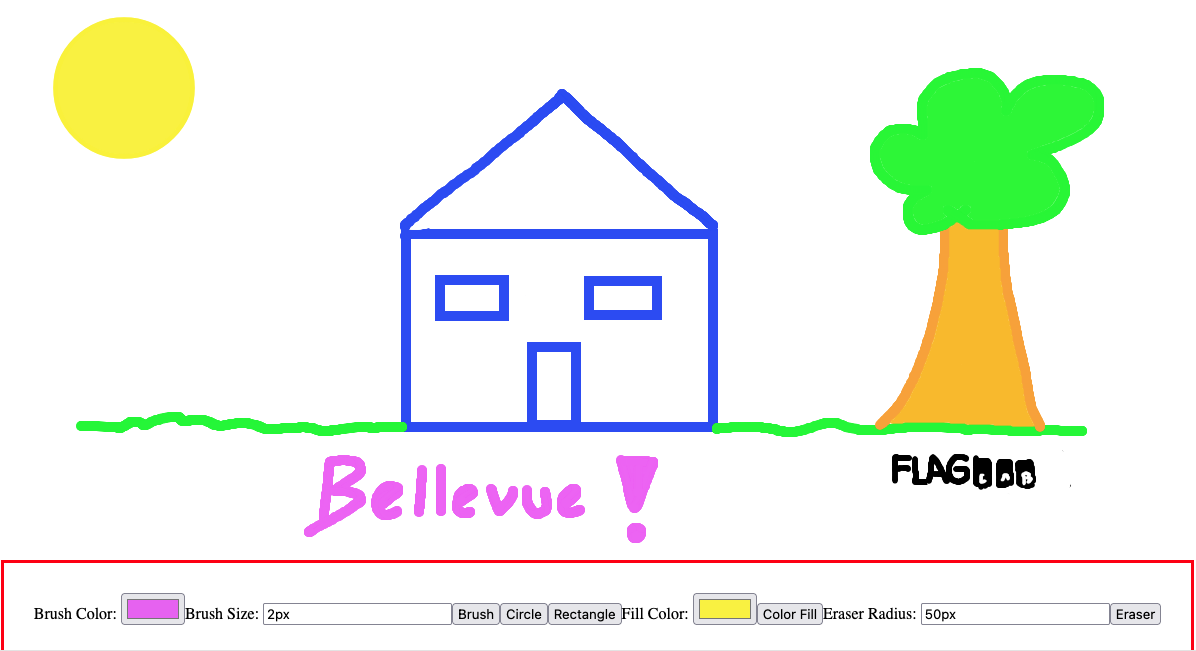
\includegraphics[width=14cm]{figures/BellevueExample}
  \caption{Bellevue}
  \label{fig:bellevue}
\end{figure}

\fref{fig:bellevue} shows a view of the Bellevue editor with its drawing tools and features.
The full implementation of the application can be found in the following repository: \url{https://github.com/slemus9/bellevue}

\section{Implementation}

The \textbf{Model} of the application is represented by the \lstinline|DrawingModel| class in \fref{lst:bellevue-model}. It contains data about
the current selected tool, the styling configuration chosen by the user and the state of the mouse interaction, among other things.

\begin{scala}[label=lst:bellevue-model, caption=Bellevue Model]
final case class DrawingModel(
    selectedTool: Tool,
    brushConfig: StyleConfig,
    colorFillConfig: ColorFillConfig,
    eraserConfig: EraserConfig,
    mouseDragging: Option[MouseDragging],
    receivedMessage: Msg
)
\end{scala}

The \lstinline|Tool| type in \fref{lst:bellevue-tool} represents a drawing tool that can be selected by the user, and it is modelled as a simple enumeration.

\begin{scala}[label=lst:bellevue-tool, caption=Bellevue drawing tools]
enum Tool:
  case Brush, ColorFill, Circle, Eraser, Rectangle
\end{scala}

The mouse interaction is represented by the \lstinline|MouseDragging| class in \fref{lst:bellevue-mouse-dragging}.
All drawing actions are performed through mouse dragging: the user clicks on any point in the canvas, then drags the mouse across it, and finally releases the mouse.
A \lstinline|MouseDragging| instance holds the starting position at which the mouse was clicked, and the latest position that was recorded while the mouse was being dragged.

\begin{scala}[label=lst:bellevue-mouse-dragging, caption=Bellevue mouse dragging modelling]
final case class MouseDragging(
    startPosition: Point,
    latestPosition: Point
)
\end{scala}

Finally, \lstinline|Msg| is a Sum Type of all types of \textbf{Messages} that can be exchanged in the application:

\begin{scala}[label=lst:bellevue-msg]
type Msg = ControlMsg | MouseMsg | ToolboxMsg

enum ControlMsg:
  case HtmlElementLoaded(id: String)
  case MapToCanvas(point: Point, toMouseMsg: Point => MouseMsg)
  case NoAction
  case ResizeCanvas

enum MouseMsg:
  case MouseDown(point: Point)
  case MouseMove(point: Point)
  case MouseUp(point: Point)

enum ToolboxMsg:
  case PickBrushSize(size: Pixels)
  case PickColor(color: RGB)
  case PickEraserRadius(radius: Pixels)
  case PickFillColor(color: RGB)
  case PickTool(tool: Tool)
  case SetCanvasImage(image: Image)
\end{scala}

The logic of the application is defined within the \textbf{Update} function. The \emph{Tyrian}~\cite{Indigoengine2025} front-end framework was used for this case study to implement Bellevue. It provides an abstraction to develop
web applications based on the Elm architecture, and the \textbf{Update} function signature is:

\begin{scala}[label=lst:bellevue-update-signature]
def update(model: DrawingModel): Msg => (DrawingModel, Cmd)
\end{scala}

Given a current \lstinline|model| and a \textbf{Message} of type \lstinline|Msg|, the \lstinline|update| function returns a new
\lstinline|DrawingModel| together with a \textbf{Command} (side effect) of type \lstinline|Cmd|, that may or may not produce a new \textbf{Message}.
Instead of explicitly dispatching all types of messages in a single pattern matching block, the \textbf{Update} function is implemented as the composition of several \textbf{Predicated Functions},
each of them describing a particular drawing interaction, that is implicitly activated as specified by their \lstinline|isActive| predicate.

For instance, \fref{lst:bellevue-brush-action} shows the definition of \lstinline|BrushAction|, a \textbf{Predicated Function} that draws into the canvas whenever the user wants to perform
a free-hand drawing using a "brush".

\begin{scala}[label=lst:bellevue-brush-action, caption=Free hand brush drawing action]
object BrushAction extends PredicatedFunction[DrawingModel, Cmd]:

  override def isActive(state: DrawingModel): Boolean =
    state.selectedTool == Tool.Brush &&
      state.receivedMessage.isInstanceOf[MouseMsg] &&
      state.mouseDragging.isDefined

  override val run: Behavior[DrawingModel, Cmd] = prevAction => model =>
    (model.receivedMessage, model.mouseDragging) match
      case (MouseMsg.MouseMove(to), Some(dragging)) =>
        val from = dragging.latestPosition
        val drawSegment = canvas.drawLineSegment(from, to)
        (model, prevAction |+| drawSegment)

      case (MouseMsg.MouseUp(to), Some(dragging)) =>
        val from = dragging.latestPosition
        val drawSegment = canvas.drawLineSegment(from, to)
        (model, prevAction |+| drawSegment)
\end{scala}

Only when the selected tool is a \lstinline|Brush| and the user is performing a mouse drag, will the
\lstinline|BrushAction| draw a small line segment between the latest position recorded and the position to which the mouse was dragged at.
Note that the \lstinline|drawSegment| side effect is being concatenated to the previous action's side effect using the |+| operator; this means
that the action of drawing a line segment will be executed alongside with whatever action was previously active.

For the drawing to be consistent, the model needs to be updated so that the \lstinline|mouseDragging| object accurately reflects the user's actions.
A separate Predicated Function can be defined just for this purpose, as shown in \fref{lst:bellevue-mouse-drag-update-action}.

\begin{scala}[label=lst:bellevue-mouse-drag-update-action, caption=Action to update the mouse dragging state]
object MouseDragUpdateAction extends PredicatedFunction[DrawingModel, Cmd]:

  override def isActive(state: DrawingModel): Boolean =
    state.receivedMessage.isInstanceOf[MouseMsg]

  override val run: Behavior[DrawingModel, Cmd] = prevAction => model =>
    model.receivedMessage match
      case MouseMsg.MouseDown(from) => (model.clickMouse(from), prevAction)
      case MouseMsg.MouseMove(to)   => (model.moveMouse(to), prevAction)
      case MouseMsg.MouseUp(_)      => (model.releaseMouse, prevAction)
\end{scala}

The \lstinline|MouseDragUpdateAction| updates the \lstinline|mouseDragging| state whenever a \lstinline|MouseMsg| was received.
Note that this action does not perform any side effects on its own, as it only returns the previous active action's side effect. The only thing it does,
is update the model in accordance to the received mouse positions. If the user clicked the mouse (\lstinline|MouseDown|), it will create a new
\lstinline|MouseDragging| instance using the mouse position as the \lstinline|startPosition|. If the user is moving the mouse around (\lstinline|MouseMove|), then it will
set the \lstinline|latestPosition| of the \lstinline|mouseDragging| state to the current mouse position. Otherwise, if the user releases the mouse (\lstinline|MouseUp|), it will
set the \lstinline|mouseDragging| state to \lstinline|None|, signaling that the mouse drag interaction ended.

\begin{scala}[label=lst:bellevue-mouse-drag-update-action-aux, caption=Complementary functions to update the mouse dragging state]
  def clickMouse(startPosition: Point) =
    copy(mouseDragging = Some(MouseDragging.init(startPosition)))

  def moveMouse(to: Point) =
    this.focus(_.mouseDragging.some.latestPosition).replace(to)

  def releaseMouse =
    copy(mouseDragging = None)
\end{scala}

Since most drawing actions are mouse dragging interactions, abstracting this behavior into a separate \lstinline|MouseDragUpdateAction| function enables better reusability.
Actions like drawing rectangles or erasing are similar to the \lstinline|BrushAction| function, and they also rely on a proper model update of the \lstinline|mouseDragging| state.
\fref{lst:bellevue-common-draw-actions-predicates} shows the activation predicates for some common drawing actions:

\begin{scala}[label=lst:bellevue-common-draw-actions-predicates, caption=Common drawing actions predicates]
// Draws rectangles
object RectangleAction extends PredicatedFunction[DrawingModel, Cmd]:

  override def isActive(state: DrawingModel): Boolean =
    state.selectedTool == Tool.Rectangle &&
      state.receivedMessage.isInstanceOf[MouseMsg]

// Draws circles
object CircleAction extends PredicatedFunction[DrawingModel, Cmd]:

  override def isActive(state: DrawingModel): Boolean =
    state.selectedTool == Tool.Circle &&
      state.receivedMessage.isInstanceOf[MouseMsg]

// Erases drawings by painting circles of the same color as the background
object EraserCanvasAction extends PredicatedFunction[DrawingModel, Cmd]:

  override def isActive(state: DrawingModel): Boolean =
    state.selectedTool == Tool.Eraser &&
      state.mouseDragging.isDefined &&
      state.receivedMessage.isInstanceOf[MouseMsg]
\end{scala}

Each function defines how to manipulate the canvas independently, but they all should receive a consistent \lstinline|mouseDragging| state.
To make sure this is the case, the functions can be composed with the \lstinline|MouseDragUpdateAction| as shown in the following code snippet:

\begin{scala}[label=lst:bellevue-draw-actions-composition, caption=Drawing actions composition]
val DrawAction: PredicatedFunction[DrawingModel, Cmd] =
  PredicatedFunction.sequence(
    PredicatedFunction.oneOf(
      BrushAction,
      CircleAction,
      EraserAction,
      RectangleAction
    ),
    MouseDragUpdateAction
  )
\end{scala}

The implementation of the remaining Bellevue features follow the same structure; canvas and state manipulation are separated into different Predicated Functions,
and they are later composed in the proper order. Finally, there is a single \lstinline|BellevueAction| function that comprises all functionality, and it is then used to define the body of the
\textbf{Update} function

\begin{scala}[label=lst:bellevue-update-function-def, caption=Bellevue Update function definition]
val BellevueAction: PredicatedFunction[DrawingModel, Cmd] =
  PredicatedFunction.oneOf(DrawAction, ...)

def update(model: DrawingModel): Msg => (DrawingModel, Cmd) =
  msg => BellevueAction.runWith(model.withMessage(msg), Cmd.None)
\end{scala}


%%
\subsection{Verification with Refinement Types}
\label{sec:verification}

A total of 15 Predicated Functions are defined to specify the \textbf{Update} function.
All of them should be composed in the right order, and there are implicit dependencies between the activation conditions of some of the functions.
While developing the case study without Refinement Types, most of the bugs introduced in the application were due to inconsistencies in the interaction between the functions.
In \fref{sec:preliminaries.cop}, we defined a layer interaction as the dependency that is formed between two layers, due to the fact that the state manipulation and Behavior of one layer, may affect the activation and Behavior of another one.
In terms of \lstinline|PredicatedFunctions|, these interactions are materialized by applying our composition functions (\lstinline|sequence| and \lstinline|orElse|), and they can result in an inconsistent behavior depending on the definition of the activation predicate and \lstinline|Behavior| of each function.
We have already seen some examples of inconsistent interactions in \fref{sec:context-scala.refined-predicated-functions}, where \lstinline|PredicatedFunctions| can be activated or deactivated due to the \lstinline|Behavior| of a previous active function.
In this section we identify two classes of errors that arise from inconsistent interactions, and we illustrate how these issues can be detected at compile-time using our approach.

The first class of identified errors, is the rendering of incorrect drawings due to incorrectly-ordered compositions.
For instance, if the \lstinline|MouseDragUpdateAction| is placed as the first function of the composition in \fref{lst:bellevue-draw-actions-composition}, some of the drawings will be inconsistent with respect to the user actions.
This is because, if a \lstinline|MouseUp| message is received, the \lstinline|releaseMouse| state modification sets the \lstinline|mouseDragging| value to \lstinline|None|, even when the other functions still need it to perform some operations in the canvas.
For example, circles would not be drawn at all, since the \lstinline|MouseUp| event marks the point where the user wants to display the final shape.
To prevent this type of errors, we can rely on the \lstinline|Chainable| type from \fref{sec:context-scala.refined-predicated-functions} to verify that the activation and state manipulation of one function, does not deactivate a subsequent function in the composition.

\begin{scala}[label=lst:enforcing-dependencies, caption=Enforcing dependencies between two Predicated Functions, escapechar=~]
final class BrushAction extends PredicatedFunction[DrawingModel, Cmd]:
  override def isActive(state: DrawingModel): Boolean =
    state.selectedTool == Tool.Brush &&
      state.receivedMessage.isInstanceOf[MouseMsg] &&
      state.mouseDragging.isDefined
  ...

final class MouseDragUpdateAction extends PredicatedFunction[DrawingModel, Cmd]:
  override def isActive(state: DrawingModel): Boolean =
    state.receivedMessage.isInstanceOf[MouseMsg]
  ...

// Compiles successfully:
val validChain = new Chainable[DrawingModel, Cmd]:
  override def first = new BrushAction
  override def second = new MouseDragUpdateAction

// Stainless produces compilation error:
val invalidChain = new Chainable[DrawingModel, Cmd]:
  override def first = new MouseDragUpdateAction
  override def second = new BrushAction
\end{scala}

In \fref{lst:enforcing-dependencies}, the \lstinline|validChain| value compiles successfully because the following typing judgement is valid:

\begin{equation}
\begin{split}
isChainable &: (previous: Cmd) \\
            &\rightarrow (state: DrawingModel) \\
            &\rightarrow unit\{BrushAction.isActive(state) \\
            &\Rightarrow MouseDragUpdateAction.isActive(BrushAction.run(previous, state).first)\}
\end{split}
\end{equation}

Recall from \fref{lst:bellevue-brush-action} that \lstinline|BrushAction| returns the previous state without modifications in all of its branches,
and thus $BrushAction.run(previous, state).first = state$, reducing the type definition to:

\begin{equation}
\begin{split}
isChainable &: (previous: Cmd) \\
            &\rightarrow (state: DrawingModel) \\
            &\rightarrow unit\{BrushAction.isActive(state) \\
            &\Rightarrow MouseDragUpdateAction.isActive(state)\}
\end{split}
\end{equation}

\noindent
Where the inner implication $BrushAction.isActive(state) \Rightarrow MouseDragUpdateAction.isActive(state)$ further reduces to:

\begin{equation}
\label{eqn:brush-mouse-drag-impl}
\begin{split}
(selectedTool = Brush & \; \wedge \; receivedMessage \; : \; MouseMsg \\
  & \; \wedge \; isDefined(mouseDragging)) \\
  & \Rightarrow receivedMessage \; : \; MouseMsg
\end{split}
\end{equation}

The \ac{SMT} solver accepts the implication from Equation \ref{eqn:brush-mouse-drag-impl} as a valid formula due to the fact that, for any propositions $A$ and $B$, the formula $A \wedge B \Rightarrow B$ (and $A \wedge B \Rightarrow A$) is a tautology.
On the contrary, \lstinline|invalidChain| does not compile because an implication in the opposite direction does not hold.
These values are static checks showing that \lstinline|BrushAction| must necessarily go before \lstinline|MouseDragUpdateAction| in the composition chain,
preventing the programmer from misordering the Predicated Functions.

This approach can be repeated for all function interactions that need to be verified. Recall from \fref{lst:bellevue-draw-actions-composition}, that \lstinline|BrushAction| is not the only function that must go before \lstinline|MouseDragUpdateAction|.
The former is also accompanied by more alternative functions inside the \lstinline|oneOf| composition, and thus, the previous dependency relation must also be guaranteed
for all of these functions. In order to achieve this, the programmer can define an auxiliary property that verifies that this implication is satisfiable for a given list of Predicated Functions, as illustrated in \fref{lst:enforcing-multiple-dependencies}.

\begin{scala}[label=lst:enforcing-multiple-dependencies, caption=Enforcing dependencies between multiple Predicated Functions, escapechar=~]
def oneOfLaw(previous: Cmd, state: DrawingModel): Boolean =
  val drawActions     = List(
    new BrushAction,
    new CircleAction,
    new ColorFillAction,
    new RectangleAction
  )
  val mouseDragUpdate = new MouseDragUpdateAction

  drawActions.forall { action =>
    action.isActive(state) ==> {
      val (newState, _) = action.run(previous, state)
      mouseDragUpdate.isActive(newState)
    }
  }.holds
\end{scala}

The second class of common mistakes consists on overspecifying some of the activation predicates. For instance, one may think that it makes sense to add the \lstinline|state.mouseDragging.isDefined| condition to the \lstinline|isActive| predicate of \lstinline|RectangleAction|, just as it was done in the \lstinline|BrushAction|'s activation predicate.
However, the \lstinline|RectangleAction| also needs to display an overlaid element to highlight the place where the rectangle will be drawn in the canvas, and this is done when \lstinline|state.mouseDragging| is equal to \lstinline|None| (as soon as the new mouse dragging interaction starts). Hence, adding the new condition will make this piece of logic
to be silently ignored, as there is no static guarantee that the \lstinline|run| function definition respects the assumptions from the \lstinline|isActive| predicate:

\begin{scala}[label=lst:malformed-rectangle-action, caption=Example bug in RectangleAction, escapechar=~]
// Example of an ill-specified predicated function for drawing rectangles
object MalformedRectangleAction extends PredicatedFunction[DrawingModel, Cmd]:

  override def isActive(state: DrawingModel): Boolean =
    state.selectedTool == Tool.Rectangle &&
      state.receivedMessage.isInstanceOf[MouseMsg] &&
      state.mouseDragging.isDefined // <-- adding this condition introduces a bug


  override val run: Behavior[DrawingModel, Cmd] = prev => model =>
    (model.receivedMessage, model.mouseDragging) match
      case (MouseMsg.MouseDown(from), None) =>
        // This piece of code is unreachable ~\label{ln:malformed-rectangle-action.unreachable}~
        (model, prev |+| overlaidRectangle.show)

      case (MouseMsg.MouseMove(to), Some(dragging)) =>
        val rectangle = Rectangle(from = dragging.startPosition, to)
        (model, prev |+| overlaidRectangle.draw(rectangle))

      case (MouseMsg.MouseUp(to), Some(dragging)) =>
        val rectangle = Rectangle(from = dragging.startPosition, to)
        val draw = canvas.drawRectangle(rectangle) |+| overlaidRectangle.hide
        (model, prev |+| draw)

      case _ => (model, prev)
\end{scala}

\fref{ln:malformed-rectangle-action.unreachable} of \fref{lst:malformed-rectangle-action} states that the piece of code that makes the overlaid rectangle visible is ignored,
because the \lstinline|run| function patten matching specifies that it should be done when \lstinline|state.mouseDragging =   None|, but the Behavior of \lstinline|MalformedRectangleAction| will only be executed when \lstinline|state.mouseDragging| is defined, directly contradicting the assumptions from the \lstinline|run| function.

Most bugs that are caused by inconsistent predicates can be detected by adding the \lstinline|isActive| predicate as a pre-condition to the \lstinline|run| function.
This way, it can be guaranteed that the \lstinline|run| function respects the assumptions from the activation predicate, and Stainless will raise an error if there are inconsistencies.
In this case, we could bring the \lstinline|isActive| assumptions to the \lstinline|run| function, and then formulate a property asserting that the overlaid rectangle should always be visible when a mouse dragging interaction starts.
\fref{ln:refined-rectangle-action.property} of \fref{lst:refined-rectangle-action} shows a property asserting that for all \lstinline|prev: Cmd| and \lstinline|model: DrawingModel| values, the \lstinline|RefinedRectangleAction| should display the overlaid rectangle whenever there is a mouse-down interaction, and the \lstinline|mouseDragging| state is set to \lstinline|None|.
This will detect the unreachable code bug encountered previously, because there is no possibility that \lstinline|overlaidRectangle.isVisible| variable will be set to true, due to the additional \lstinline|state.mouseDragging.isDefined| precondition

\begin{scala}[label=lst:refined-rectangle-action, caption=Enforcing activation assumptions in the RectagleAction, escapechar=~]
final class RefinedRectangleAction extends PredicatedFunction[DrawingModel, Cmd]:

  override def isActive(state: DrawingModel): Boolean =
    state.selectedTool == Tool.Rectangle &&
      state.receivedMessage.isInstanceOf[MouseMsg] &&
      state.mouseDragging.isDefined // <-- adding this condition introduces a bug

  override def run(prev: Cmd, model: DrawingModel): Cmd =
    require(this.isActive(model)) // <-- add precondition
    ...

// This property will fail because the precondition is not met
def overlaidRectVisibleWhenMouseDragging( ~\label{ln:refined-rectangle-action.property}~
    prev: Cmd,
    model: DrawingModel
    mouseDown: MouseMsg.MouseDown
): Boolean =
  val action = new RefinedRectangleAction
  val inputModel  = model.copy(
    selectedTool = Tool.Rectangle,
    receivedMessage = Msg.Mouse(mouseDown),
    mouseDragging = None()
  )
  // The following call violates the activation precondition:
  val (_, result) = action.run(prev, inputModel)
  result.overlaidRectangle.isVisible
\end{scala}

Though these bugs may seem simple and easy to avoid, they can be hard to detect due to the high decoupling between activation and behavior.
As the application's complexity increases and new Predicated Functions are defined, the difficulty of finding these simple bugs increases, since there may be more interactions that need to be taken into account.


%%
\subsection{Discussion}
\label{sec:discussion}

Throughout the development of this case study, various challenges when creating \ac{COP} applications were evidenced,
and an alternative approach was explored to mitigate those challenges using Refinement Types.
Some of the main findings encountered while designing and implementing this approach are:

\begin{itemize}
  \item
    Refinement Types are a convenient verification tool because they are integrated with the language in which the application is being implemented, allowing the programmer to verify the actual code that is going to be executed.
    However, there were some limitations while trying to integrate with existing code and libraries for this case study. Though Stainless offers an \lstinline|@extern| annotation to do this incorporation, some Scala compiler errors were encountered during type checking.
    For instance, it was not possible to use the Tyrian framework's \lstinline|Cmd[F, A]| type inside the signature of the \lstinline|PredicatedFunction|

  \item
    Due to the difficulty of integrating with existing code, a separate notion of \textbf{Commands} had to be implemented in the Stainless \emph{Pure Scala} language subset, which then had to be translated to the Tyrian framework's \lstinline|Cmd[F, A]| type.
    This translation process introduces an additional layer of code in the application that is not verified, so further testing or verification needs to be done to cover it.
    Unfortunately, this opposes the expectation that was held at the beginning of this work, regarding a seamless code integration when using Refinement Types.

  \item
    Refinement Types were successfully used to verify some of the main interactions between Predicated Functions in this case study.
    Though the defined properties and dependency relations are specific to the needs of this particular application, it is believed that Refinement Types (and Stainless) is a sufficiently robust tool to reason about many other properties of \ac{COP} programs.

  \item
    The design choices that were made to implement \lstinline|PredicatedFunctions| and the \text{Bellevue} application facilitated the process of formal verification.
    The \lstinline|PredicatedFunction| composition naturally fits into the Elm architecture, since the signature of the \textbf{Update} function is very similar to the definition of a \lstinline|PredicatedFunction|.
    The Elm architecture, in turn, made it easier to apply Refinement Types, as we take on a Purely Functional approach of implementing the application, which is a paradigm well suited for Stainless.

  \item
    The \lstinline|Chainable| abstraction is enough to verify dependencies between two Predicated Functions, however it is not very ergonomic as the programmer has to manually construct these instances for all pair of functions that need to be verified.
    Furthermore, for composition chains longer than two functions, a transitive relation between \lstinline|Chainable|s must be established for full correctness. An attempt was made to formulate a more ergonomic \lstinline|Chainable| abstraction for multiple functions while enforcing transitivity, but unfortunately it was not completed for this case study.

  \item
    Another disadvantage of the \lstinline|Chainable| abstraction, is that is not integrated yet with the \lstinline|sequence| and \lstinline|oneOf| composition functions. So, if the programmer forgets to construct a \lstinline|Chainable| instance, these composition functions can still be used to potentially construct unsound Predicated Functions.
    A more principled approach would be to define \lstinline|andThen| and \lstinline|orElse| operations in such a way that they receive a \lstinline|Chainable| instance as an argument, which serves as an \emph{evidence} that two functions can be composed because the given dependency property holds.
    This way, it is mandatory for the programmer to verify these dependency relations before building compositions.

  \item
    More work can be done to verify more complex properties in this application regarding state transitions. For example, there is a \lstinline|ColorFill| action that contains the logic of flood-filling a closed area with a selected color.
    This Predicated Function requires the current bitmap of the canvas to be given (i.e. there is a \lstinline|.canvasImage.isDefined| condition in the activation predicate). It would be desirable to verify that the \lstinline|ColorFillAction| \emph{always} receives such bitmap when the selected tool is equal to \lstinline|Tool.ColorFill|.
    The reason why this property is harder to check with the current abstractions, is because the action that sets the bitmap is not directly chained with the \lstinline|ColorFillAction|, since they happen at two separate time instances.
    A way to tackle this would be to extend the abstractions developed in this work so that the programmer reason about state transitions, and possibly base such implementation in Temporal Logic.
\end{itemize}


\endinput


% !TEX root = ./../main.tex

\section{Related Work}
\label{sec:related-work}

We now explore existing proposals related to our work in three directions. Approaches that use type 
systems to verify \ac{COP} programs, existing verification approaches that use Refinement Types
(\eg in Reactive Programming, a paradigm used to implement \ac{COP}~\cite{watanabe14,leger23}),
and verification techniques in domains closely related to \ac{COP} such as Self-Adaptive Systems
and Actor Systems~\cite{watanabe14}.


%%
\subsection{Use of Type Systems in \acl{COP}}
\label{sec:types-cop}

There exist several Type-based solutions to verify the properties of \ac{COP} programs.
~\citet{aotani15} propose an abstraction to guarantee that layers relying on an imperative activation 
mechanism do not call methods on other layers that are inactive. This is done by modeling layer 
activation with Typestates. A Typestate denotes the run-time state of a resource so that we can 
determine when an operation can be applied to the resource, and how it changes the resource's state.
In particular, there are two Typestates in the approach. The type $\uparrow L$, denotes that layer 
$L$ is active, and the type $\downarrow L$, denotes that layer $L$ is inactive. This way of tracking the 
state of layers allows us to define the \scode{activate} and \scode{deactivate} operations in a way that 
they can only be applied to a consistent state, \ie the \scode{activate} function can only be applied to  
layers with type $\downarrow L$, and the \scode{deactivate} function can only be applied to layers with 
type $\uparrow L$.
The problem solved with Typestates focuses only on the consistency of activation/deactivation 
operations, and not on the interaction between layers. Using Refinement Types we can have the same 
guarantees when we add the \scode{isActive} predicate as a precondition to the \scode{run} function.

JCop~\cite{inoue14} has Type-level constructions to verify layer interactions, by explicitly stating the 
dependency between two layers in their type definition. For instance, given two layers \scode{L1} and 
\scode{L2}, the programmer can specify a dependency between them in JCop by using the 
\scode{requires} keyword, ensuring that \scode{L1} is always activated before \scode{L2} 
(\scode{public layer L1 requires L2}).
This approach, however, only works well for imperative activation mechanisms as it was briefly 
discussed in \fref{sec:cop}. No alternatives have been found to statically verify layer interactions with 
declarative activation mechanism, and our approach with Refinement Types puts forward a viable 
solution to do so.


%%
\subsection{Verification of Reactive Programs Using Refinement Types}
\label{sec:verification-reactive-programming}

in the \ac{RP} paradigm programs \emph{react} to values that vary through time.
It is common to find applications that require software adaptability (such as IoT systems or web 
applications) implemented with \ac{RP}. For example, Bellevue relies on an abstraction that dictates how 
the program should react to changes in the state (the \scode{DrawingModel}). The \scode{update} 
function, in particular, is the main source of the relevant time-varying values (state and messages).

Software verification is used in \ac{RP} to have a precise description of the desired run-time behavior of 
a reactive program. The work by~\citet{chen24} is an example of using Refinement Types to verify \ac{RP} programs. Refinement Types are used 
to describe post-conditions for functions that process time-varying data (\ie streams), as well as to 
declare invariants over such data. A type system is developed extending the Refinement Types 
language with predicates drawn from Linear Temporal Logic. These predicates are used to reason 
about the behavior of data streams. In particular, the type system introduces the 
$\{ w : b \; | \; \square \; \phi \}$ refinement to specify that $\phi$ must hold for all values of the stream 
$w$ from the current instant of time onwards, and the $\{ w : b \; | \; \bigcirc \; \phi \}$ refinement to 
describe that $\phi$ must hold in the next time instant. The resulting system allows programmers to 
formally verify, simulate and deploy Cyber-Physical Systems.

The use of Refinement Types to verify Cyber-Physical Systems is closely related to our proposal. First, 
Cyber-Physical Systems are an application domain of \ac{COP}, often benefiting from dynamic 
adaptation. Second, as mentioned before, there are \ac{COP} languages based on \ac{RP}, so the use 
of Refinement Types in an \ac{RP} context can translate naturally to reactive-based \ac{COP} 
languages. 

Moreover over, we note that our approach could benefit from this Temporal Logic extension to prove 
more sophisticated properties. For example, to prove that the \scode{ColorFillAction} always receives 
the canvas bitmap if, at some previous point in time, the user selected the \scode{ColorFill} tool, is an 
specification that could be written using Temporal Logic.


%%
\subsection{Verification in Actor Systems for Software Adaptability}
\label{sec:verification-actors}

EnsembleS~\cite{harvey21} is an actor-based language based on Multiparty Session Types to 
define an verify programs that can \emph{adapt} their behavior in response to the operating 
environment. \emph{Adaptability} in this context refers to the ability of sensing the environment and 
respond by \emph{discovering} new components, \emph{replacing} behavior or \emph{communicating} 
information. EnsembleS defines actors as single-threaded entities that do not share state, and have a 
channel-based message communication between each other. The programmer is able to create static 
topologies, where all participants are present throughout the duration of a session, as well as dynamic 
topologies where participants can connect or disconnect at a given point in the session.

The main contribution of this work is the static verification of dynamic interaction and replacement of 
functionality, which cannot be guaranteed by using Multiparty Session Types alone. EnsembleS offers 
the \scode{link} and \scode{unlink} statements to enable dynamic connectivity,  and verifies that the 
replacement of functionality does not violate the communication protocol that is already established by 
the Session Type. 
It is possible to consider an alternative formulation to verify \ac{COP} programs with Session Types, 
where one can granularly specify the sequence of steps of a program with Session Types, and model 
(de)activation with a replacement mechanism similar to the one defined for EnsambleS. This would 
greatly differ from the Refinement Types alternative, as the programmer would need to explicitly 
specify all steps in the flow of the \ac{COP} program. However, such an approach could suffer from 
the state explosion problem of interactions between adaptations.


%%
\subsection{Verification in Self-Adaptive Systems}
\label{sec:verification-as}

\citet{weyns12} present a survey of the existing formal methods for Self-Adaptive Systems. The 
survey compiles various studies from conferences and journals, and discusses the main methods that 
have been used to formally reason about such systems, as well as the main program properties of 
interest to the researchers.
The main modeling language for property specification is algebra, but a very limited set of studies 
actually used automated reasoning to evidence the validity of such properties. The ones that do, often 
use Model Checking or Theorem Proving to a lesser extent. Liveness, safety, and reachability are 
some of the common properties of interest, but most studies focus on verifying behavior specific to the 
use case or area of self-adaptation.
One of the main remarks from the survey, is that there are not many studies that make use of software 
verification in this area, and that there is a need of light-weight and pluggable verification 
tools~\cite{weyns12}. As validated from our approach, Refinement Types could be a good candidate in 
that regard, as they provide a seamless and pluggable integration of property specification within the 
same language in which the application is being developed.
Furthermore, Refinement Types shares some similarities with model checking in the sense that 
Refinement Types use \ac{SMT} solvers to validate the verification constraints, with model checkers 
using SAT solvers to check the satisfiability of a propositional formula that represents the program 
traces of the finite state system under verification~\cite{armando06}.


\endinput


% !TEX root = ./../main.tex

\section{Conclusion and Future Work}
\label{sec:conclusion}

The objective of this work is to explore the use of Refinement Types to formally reason about \ac{COP} 
programs, and manage the possible inconsistencies or incompleteness that may arise at run time, in 
response to the interaction between layers. Refinements Types are chosen due to their ease of 
integration with existing programming languages, and their powerful features that allow the programmer 
to formulate functions' pre-conditions and post-conditions, as well as to prove mathematical statements 
about the program's functionality. There are many ways to implement \ac{COP}, however, expressing it 
as a set of partial functions that can be composed together to incrementally build programs, significantly 
simplifies the process of writing and verifying \ac{COP} applications.

To validate the usefulness of Refinement Types in verifying \ac{COP} programs, we use the Bellevue 
graphical editor, as a validating case study implemented in two iterations. The first iteration evidences 
errors caused by unforeseen interactions between the layers in \ac{COP} programs. Modifications to the 
program, such as changing the composition order of predicated functions, or adding a condition to the 
activation predicates, can introduce bugs that are hard to detect, as the decoupling between application 
logic and layer activation makes it harder to reason about the program. The second iterations uses
Refinement Types, with the abstractions to mange them, making the bugs explicit and statically 
verifiable. Enforcing the assumptions stated in the activation predicates into the application's logic, 
inconsistencies and incompleteness can be avoided while defining the functions and their composition. 
Once this is guaranteed, the programmer can then specify more complex properties to verify the 
interactions between functions by describing the dependencies between them in terms of activation and 
state manipulation.

As presented in \fref{sec:discussion}, the \scode{PredicatedFunction} and \scode{Chainable} 
abstractions could be improved, and more work could be done for verifying properties that involve 
states in different time instants. In particular, there are two main possibilities to improve this work.
First, we can make the \scode{andThen} and \scode{orElse} functions depend on a \scode{Chainable} 
argument (or a similar abstraction), in such a way that we disallow composing two functions unless there 
is evidence that the two functions can in fact be composed (in this case, by virtue of the 
\scode{isChainable} property). Currently, if programmers omit a \scode{Chainable} instance to verify a 
layer interaction, they can still compose the layers; the composition functions are unrestricted. Achieving 
this level of abstraction is challenging, because there may be other properties besides 
\scode{isChainable} that we would like to specify as a pre-requirement for composing two functions.
Hence, this new \scode{andThen} function would need to receive arbitrarily user defined predicates, 
instead of constant ones like the \scode{isChainable} predicate.
Second, extending the current abstractions would open the possibility to specify properties about the 
state at different points in time. We discussed in \fref{sec:discussion}, that a good example of this would 
be to statically guarantee conditions of a predicated behavior with respect to specific events 
(\eg activation of a layer) at a previous (not necessarily adjacent) time.  A potentially good approach 
would be to use Temporal Logic with Refinement Types.


\endinput




%% $Id: responses.tex 
% !TEX root = main.tex

\newpage

\appendix

\clearpage

\subsection{Response Letter}


As required by the reviewing process, we are submitting this response letter along with a revised 
version of our paper entitled \textsl{Flik: A Back-in-time Debugger for Reinforcement Learning Programs}. For convenience, the letter is formatted as an appendix of the paper.

We would like to thank our anonymous reviewers for their efforts in reviewing our submission and 
for their useful and detailed suggestions to improve it. We have considered all remarks carefully, and 
addressed them to the best of our possibilities.

There are \thetotalremarks~ different remarks for this iteration of the paper, for which we have 
effectively answered \thetotalresponses, 
while \thetotalunsolved ~are blocked or require further feedback from the reviewers. 
Each remark 
is followed by our response and an explicit status indication:

\begin{itemize}[nosep,label=--] 
	\item \revtotal{solved} \statussolved 
	\item \revtotal{future} \statusfuture
	\item \revtotal{clarify} \statusclarify\footnote{We clarify the question made by the reviewer} 
	\item \revtotal{reconsider} \statusreconsider\footnote{We ask the reviewer to reconsider the remark in the light of arguments and clarifications we provide in the response.} 
	\item \revtotal{blocked} \statusblocked\footnote{We could not accommodate the remark in the text due to blocking constraints.} 
	\item \revtotal{feedback} \statusfeedback\footnote{We answered the remark to our best interpretation. We are unsure about what the reviewer meant.} 	
\end{itemize}

The remarks with specific changes in the paper have a reference to the location in the paper 
where the solution is found. These solutions are marked with the 
\includegraphics[width=0.03\textwidth]{./figures/fix.pdf} icon in the paper margin for easy 
identification. Additionally, in the margin we point to the specific remark(s) the modification 
is addressing.


%%
\subsection{Review \#1}



\begin{remark} \label{rem:intro}
The introduction is overly technical.
\end{remark}
\begin{solved}
We rewrote the whole introduction to have a more abstract presentation of the motivation, and reduce its technicality (\fref[vario]{par:intro}). All the technical details have been moved to a new sections providing the background on \ac{RL} (\fref{sec:rl-background} - \fref[vario]{par:background})  
\end{solved}



\endinput


%%
% !TEX root = ../main.tex
\bibliographystyle{cas-model2-names}
%\biboptions{sort&compress}
\bibliography{local,bib/general, bib/compsci, bib/learning, bib/strings}
%\printbibliography


\end{document}


\endinput

